\documentclass[10pt]{article}
\renewcommand{\baselinestretch}{1.8}

\usepackage[letterpaper, margin=1in]{geometry}
\usepackage{tikz-qtree}
\usepackage{algorithm}
\usepackage{algpseudocode}
\makeatletter
\renewcommand{\ALG@beginalgorithmic}{\footnotesize}
\makeatother
\usepackage{graphicx}
\usepackage{subcaption}
%\usepackage{showkeys}
\usepackage{hyperref}
\usepackage{amsmath}
\usepackage{relsize}
\usepackage{enumitem}
\usepackage{bold-extra}

\usepackage{multicol}
\setlength\columnsep{24pt}

\algnewcommand\algorithmicforeach{\bf{for each}}
\algdef{S}[FOR]{ForEach}[1]{\algorithmicforeach\ #1\ \algorithmicdo}

\algdef{S}[FUNCTION]{Function}
   [3]{{\tt{\sl{#1}}} {\tt{#2}}\ifthenelse{\equal{#3}{}}{}{\tt{(#3)}}}
  
\algdef{E}[FUNCTION]{EndFunction}
   [1]{\algorithmicend\ \tt{{#1}}}

\algrenewcommand\Call[2]{\tt{{#1}\ifthenelse{\equal{#2}{}}{}{(#2)}}}
   
\newcommand\keywordfont{\sffamily\bfseries}
\algrenewcommand\algorithmicend{{\keywordfont end}}
\algrenewcommand\algorithmicfor{{\keywordfont for}}
\algrenewcommand\algorithmicforeach{{\keywordfont for each}}
\algrenewcommand\algorithmicdo{{\keywordfont do}}
\algrenewcommand\algorithmicuntil{{\keywordfont until}}
\algrenewcommand\algorithmicfunction{{\keywordfont function}}
\algrenewcommand\algorithmicif{{\keywordfont if}}
\algrenewcommand\algorithmicthen{{\keywordfont then}}
\algrenewcommand\algorithmicelse{{\keywordfont else}}
\algrenewcommand\algorithmicreturn{{\keywordfont return}}

\renewcommand\thealgorithm{}
\newcommand{\setalglineno}[1]{%
  \setcounter{ALC@line}{\numexpr#1-1}}

\newcommand{\sub}[1]{\textsubscript{#1}}
\renewcommand{\tt}[1]{\texttt{#1}}
\renewcommand{\sl}[1]{\textsl{#1}}
\renewcommand{\it}[1]{\textit{#1}}
\renewcommand{\sc}[1]{\textsc{#1}}
\renewcommand{\bf}[1]{\textbf{#1}}
\newcommand{\nf}[1]{{\normalfont{\texttt{#1}}}}
\newcommand{\cmt}[1]{\Comment{#1}}
\newcommand{\head}{head}
\newcommand{\size}{size }

\usepackage{amsmath,amssymb,amsthm}
\newtheorem{theorem}{Theorem}
\newtheorem{lemma}[theorem]{Lemma}
\newtheorem{corollary}[theorem]{Corollary}
\newtheorem{observation}[theorem]{Observation}
\theoremstyle{definition}
\newtheorem{definition}[theorem]{Definition}
\newtheorem{invariant}[theorem]{Invariant}


\begin{document}
\title{A Wait-free Queue with Polylogarithmic Step Complexity}
\author{Hossein Naderibeni \\supervised by Eric Ruppert}
\maketitle

\begin{abstract}
In this work, we are going to introduce a novel lock-free queue implementation.
Linearizability and lock-freedom are standard requirements for designing shared data structures. All existing linearizable, lock-free queues in the literature have a common problem in their worst case called CAS Retry Problem. Our contribution is solving this problem while outperforming the previous algorithms.
\end{abstract}

\tableofcontents
\pagebreak
\section{Introduction}
Shared data structures have become an essential field in distributed algorithms research.
We are reaching the physical limits of how many transistors we can place on a CPU core. The industry solution to provide more computational power is to increase the number of cores of the CPU. This is why distributed algorithms have become important. It is not hard to see why multiple processes cannot update sequential data structures designed for one process. For example, consider two processes trying to insert some values into a sequential linked list simultaneously. Processes $p,q$ read the same tail node, $p$ changes the next pointer of the tail node to its new node and after that $q$ does the same. In this run, $p$'s update is overwritten. One solution is to use locks; whenever a process wants to do an update or query on a data structure, the process locks it, and others cannot use it until the lock is released. Using locks has some disadvantages; for example, one process might be slow, and holding a lock for a long time prevents other processes from progressing. Moreover, locks do not allow complete parallelism since only the one process holding the lock can make progress. 


The question that may arise is, ``What properties matter for a lock-free data structure?'', since executions on a shared data structure are different from sequential ones, the correctness conditions also differ. To prove a concurrent object works perfectly, we have to show it satisfies safety and progress conditions. A \textit{safety condition} tells us that the data structure does not return wrong responses, and a \textit{progress property} requires that operations eventually terminate.


The standard safety condition is called \textit{linearizability}, which ensures that for any concurrent execution on a linearizable object, each operation should appear to take effect instantaneously at some moment between its invocation and response. Figure \ref{fig::goodexample} is an example of an execution on a linearizable  queue that is initially empty. The arrow shows time, and each rectangle shows the time between the invocation and the termination of an operation. Since \texttt{Enqueue(A)} and \texttt{Enqueue(B)} are concurrent, \texttt{Enqueue(B)} may or may not take effect before \texttt{Enqueue(A)}. The execution in Figure \ref{fig::badexample} is not linearizable since \texttt{A} has been enqueued before \texttt{B}, so it has to be dequeued first.

\begin{figure}[hbt]
  \center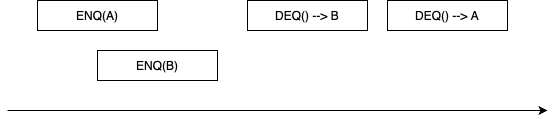
\includegraphics[scale=0.5]{pics/good}
  \caption{\label{fig::goodexample}An example of a linearizable execution. Either \texttt{Enqueue(A)} or \texttt{Enqueue(B)} could take effect first since they are concurrent.}
\end{figure}

\begin{figure}[hbt]
  \center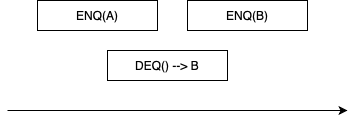
\includegraphics[scale=0.5]{pics/bad}
  \caption{\label{fig::badexample}An example of an execution that is not linearizable. Since \texttt{Enqueue(A)} has completed before \texttt{Enqueue(B)} is invoked the \texttt{Dequeue()} should return \texttt{A} or nothing.}
\end{figure}


There are various progress properties; the strongest is wait-freedom, and the more common is lock-freedom. An algorithm is \textit{wait-free} if each operation terminates after a finite number of its own steps. We call an algorithm \textit{lock-free} if, after a sufficient number of steps, one operation terminates. A wait-free algorithm is also lock-free but not vice versa; in an infinite run of a lock-free algorithm there might be an operation that takes infinitely many steps but never terminates.

A queue stores a sequence of elements and supports two operations, enqueue and dequeue. \texttt{Enqueue(e)} appends element \texttt{e} to the sequence stored. \texttt{Dequeue()} removes and returns the first element among in the sequence. If the queue is empty it returns \texttt{null}. In section 2 we talk about previous queues and their common problems. We also talk about polylogarithmic construction of shared objects.

Jayanti~\cite{DBLP:conf/podc/Jayanti98a} proved an $\Omega(\log p)$ lower bound on the worst-case shared-access time complexity of $p$-process universal constructions. He also introduced~\cite{DBLP:conf/podc/ChandraJT98} a construction that achieves $\textsc{O}(\log^2 p)$ shared accesses. Here, we first introduce a universal construction using $\textsc{O}(\log p)$ CAS operations~\cite{DBLP:conf/fsttcs/JayantiP05}. In section 3 we introduce a polylogarithmic step wait-free universal construction. Our main ideas in of the universal construction also appear in our Queue Algorithm (\ref{algQ}). The main short come of our universal construction is using big CAS objects. We use the universal construction as a stepping stone towards our queue algorithm, so we will not explain it in too much detail.

In section 4 we introduce a concurrent wait-free datastructure, to agree on the order of the operations invoked on some processes.

In section 5 we introduce our main work, the queue; prove its linearizability and wait-freeness.

\pagebreak
\section{Related Work}
\subsection{List-based Queues}
In the following paragraphs, we look at previous lock-free queues.
Michael and Scott~\cite{DBLP:conf/podc/MichaelS96} introduced a lock-free queue which we refer to as the MS-queue. A version of it is included in the standard Java Concurrency Package. Their idea is to store the queue elements in a singly-linked list (see Figure~\ref{fig::msq}). Head points to the first node in the linked list that has not been dequeued, and Tail points to the last element in the queue. To insert a node into the linked list, they use atomic primitive operations like \texttt{LL/SC} or \texttt{CAS}. If $p$ processes try to enqueue simultaneously, only one can succeed, and the others have to retry. This makes the amortized number of steps to be $\Omega(p)$ per enqueue. Similarly, dequeue can take $\Omega(p)$ steps.

\begin{figure}[hbt]
  \center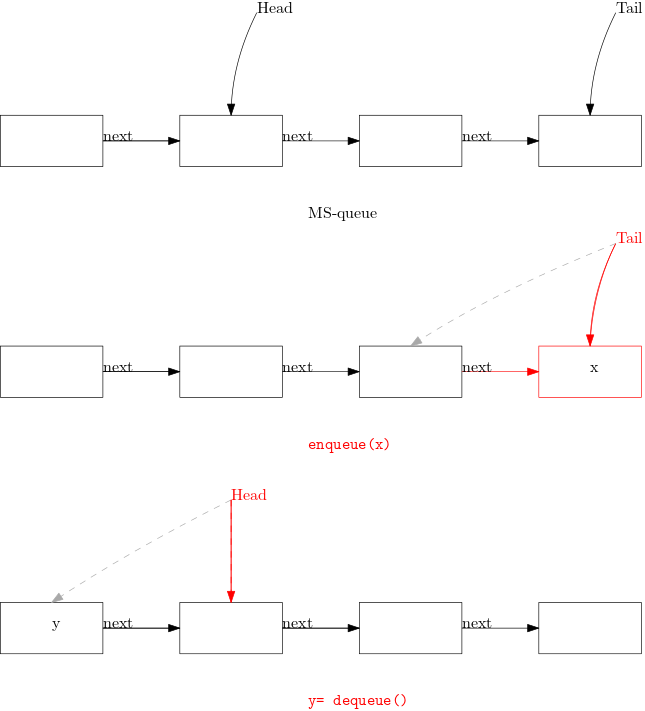
\includegraphics[scale=0.4]{pics/msqueue}
  \caption{\label{fig::msq}MS-queue structure, enqueue and dequeue operations. In the first diagram the first element has been dequeued. Red arrows show new pointers and gray dashed arrows show the old pointers.}
\end{figure}


Moir, Nussbaum, and Shalev~\cite{DBLP:conf/spaa/MoirNSS05} presented a more sophisticated queue by using the elimination technique. The elimination mechanism has the dual purpose of allowing operations to complete in parallel and reducing contention for the queue. An Elimination Queue consists of an MS-queue augmented with an elimination array. Elimination works by allowing opposing pairs of concurrent operations such as an enqueue and a dequeue to exchange values when the queue is empty or when concurrent operations can be linearized to empty the queue. Their algorithm makes it possible for long-running operations to eliminate an opposing operation. The empirical evaluation showed the throughput of their work is better than the MS-queue, but the worst case is still the same; in case there are $p$ concurrent enqueues, their algorithm is not better than MS-queue. 

Hoffman, Shalev, and Shavit~\cite{DBLP:conf/opodis/HoffmanSS07} tried to make the MS-queue more parallel by introducing the Baskets Queue. Their idea is to allow more parallelism by treating the simultaneous enqueue operations as a basket. Each basket has a time interval in which all its nodes' enqueue operations overlap. Since the operations in a basket are concurrent, we can order them in any way. Enqueues in a basket try to find their order in the basket one by one by using \texttt{CAS} operations. However, like the previous algorithms, if there are still $p$ concurrent enqueue operations in a basket, the amortized step complexity remains $\Omega(p)$ per operation.

\begin{figure}[hbt]
  \center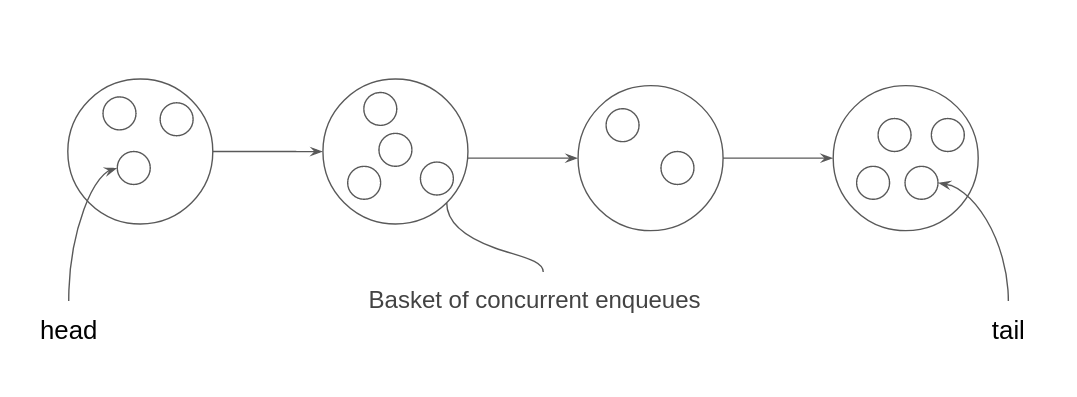
\includegraphics[scale=0.3]{pics/baskets}
  \caption{Baskets queue idea. There is a time that all operations in a basket were running concurrently, but only one has succeeded to do \texttt{CAS}. To order the operations in a basket, the mechanism in the algorithm for processes is to \texttt{CAS} again. The successful process will be the next one in the basket and so on.}
\end{figure}

Ladan-Mozes and Shavit~\cite{DBLP:journals/dc/Ladan-MozesS08} presented an Optimistic Approach to Lock-Free FIFO Queues. They use a doubly-linked list and do fewer \texttt{CAS} operations than MS-queue. But as before, the worst case is when there are $p$ concurrent enqueues which have to be enqueued one by one. The amortized worst-case complexity is still $\Omega(p)$ \texttt{CAS}es.

Hendler et al.~\cite{DBLP:conf/spaa/HendlerIST10} proposed a new paradigm called flat combining. Their queue is linearizable but not lock-free. Their main idea is that with knowledge of all the history of operations, it might be possible to answer queries faster than doing them one by one. In our work we also maintain the whole history. They present experiments that show their algorithm performs well in some situations.

Gidenstam, Sundell, and Tsigas~\cite{DBLP:conf/opodis/GidenstamST10} introduced a new algorithm using a linked list of arrays. Global head and tail pointers point to arrays containing the first and last elements in the queue. Global pointers are up to date, but head and tail pointers may be behind in time. An enqueue or a dequeue searches in the head array or tail array to find the first unmarked element or last written element (see~Figure~\ref{fig::sundell}). Their data structure is lock-free. Still, if the head array is empty and $p$ processes try to enqueue simultaneously, the step complexity remains $\Omega(p)$.

\begin{figure}[hbt]
  \center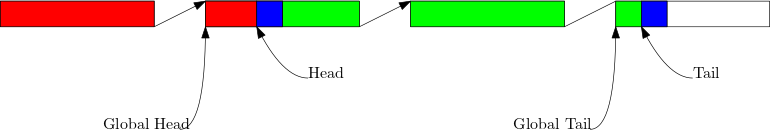
\includegraphics[scale=0.5]{pics/sundell}
    \caption{\label{fig::sundell}Global pointers point to arrays. Head and Tail elements are blue, dequeued elements are red and current elements of the queue are green.}
\end{figure}

Kogan and Petrank~\cite{DBLP:conf/ppopp/KoganP11} introduced wait-free queues based on the MS-queue and use Herlihy's helping technique to achieve wait-freedom. Their step complexity is $\Omega(p)$ because of the helping mechanism.

%todo: comparison
%Milman et al.~\cite{DBLP:conf/spaa/MilmanKLLP18} designed BQ: A Lock-Free Queue with Batching. Their idea of batching allows a sequence of operations to be submitted as a batch for later execution. It supports a new notion introduced by the authors called Extended Medium Futures Linearizability.

%Nikolaev and Ravindran~\cite{DBLP:journals/corr/abs-2201-02179} wCQ to be completed.
In the worst-case step complexity of all the list-based queues discussed above, there is a $p$ term that comes from the case all $p$ processes try to do an enqueue simultaneously. Morrison and Afek call this the \textit{CAS retry problem}~\cite{DBLP:conf/ppopp/MorrisonA13}. It is not limited to list-based queues and array-based queues share the CAS retry problem as well~\cite{DBLP:conf/spaa/TsigasZ01,DBLP:conf/icdcn/Shafiei09,DBLP:conf/iceccs/ColvinG05} . We are focusing on seeing if we can implement a queue in sublinear steps in terms of $p$ or not.

\subsection{Universal Constructions}
Herlihy discussed the possibility of implementing shared objects from other objects~\cite{10.1145/114005.102808}. A \textit{universal construction} is an algorithm that can implement a shared version of any given sequential object. We can implement a concurrent queue using a universal construction. Jayanti proved an $\Omega(\log p)$ lower bound on the worst-case shared-access time complexity of $p$-process universal constructions~\cite{DBLP:conf/podc/Jayanti98a}. He also introduced a construction that achieves $\textsc{O}(\log^2 p)$ shared accesses~\cite{DBLP:conf/podc/ChandraJT98}. His universal construction can be used to create any data structure, but its implementation is not practical because of using unreasonably large-sized \texttt{CAS} operations.

Ellen and Woelfel introduced an implementation of a Fetch\&Inc object with step complexity of $O(\log p)$ using $O(\log n$)-bit \texttt{LL/SC} objects, where $n$ is the number of operations~\cite{10.1007/978-3-642-41527-2_20}. Their idea has similarities to Jayanti's construction, and they represent the value of the Fetch\&Inc using the history of successful operations. 

%FIFO queues have a wide range of use in OS and applications. The current state-of-the-art queues are implemented using linked lists; that's why they have factor p in their time complexity.

%\href{https://docs.google.com/spreadsheets/d/1cL1tgXXdljkh462sMwkTVMHH_k0MBTmslIVM3xA5VS4/edit#gid=0}{Table of previous works}

%There is a connection between queues and universal constructions. We can implement a universal construction using a queue. We can store operations in the shared queue and compute operations' responses using the queue's content. Some impractical universal constructions are using big words as "...".

\subsection{Attiya Fourier Lower Bound}
\pagebreak

\pagebreak
\section{Queue Implementation} \label{DescriptQ}

In our model there are $p$ processes doing \nf{Enqueue} and \nf{Dequeue} operations on a queue concurrently. We design a linearizable wait-free queue with $O(\log^2 p +\log q)$ steps per operation, where $q$ is the number of elements in the queue at the time of linearization. We avoid the $\Omega(p)$ worst-case step complexity of existing shared queues based on linked lists or arrays, which suffer from the CAS Retry Problem. 

Jayanti and Petrovic introduced a wait-free poly-logarithmic multi-enqueuer single-dequeuer queue~\cite{DBLP:conf/fsttcs/JayantiP05}. We use their idea of having a tournament tree among processes to agree on the linearization of operations to design a a polylogarithmic multi-enqueuer multi-dequeuer queue. Unlike their work, our algorithm does not put a limit on the number of concurrent dequeuers. 

There is a shared binary tree among the processes (see Figure~\ref{fig::blocktree}) to agree on one total ordering of the operations invoked by processes. Each process has a leaf in which the operations invoked by the process are stored in order. When a process wishes to do an operation it appends the operation to its leaf and tries to propagate its new operation up to the tree's root. Each node of the tree keeps an ordering of operations propagated up to it. All processes agree on the sequence of operations in the root and this ordering is used as the linearization ordering. 
\begin{figure}[hbtp]
\begin{center}
\Tree [ [ [ $P_1$ $P_2$ ] [ $P_3$ $P_4$ ] ]
          [ [ $P_5$ $P_6$ ] [ $P_7$ $P_8$ ] ] ]
\end{center}
\caption{\label{fig::blocktree}Each of the processes $P_1,P_2,...,P_p$ has a leaf and in each node there is an ordering of operations stored. Each process tries to propagate its operations up to the root, which stores a total ordering of all operations.}  
\end{figure}

To propagate operations to a node $n$ in the tree, a process observes the operations in both of $n$'s children that are not already in $n$, merges them to create an ordering and then tries to append the ordering to the sequence stored in $n$. We call this procedure \tt{$n$.Refresh()} (see Figure \ref{fig::propagstep}). A \nf{Refresh} on $n$ with a successful append helps to propagate their operations up to the $n$. We shall prove that if a process invokes \tt{Refresh} on the node $n$ two times and fails to append the new operations to $n$ both times, the operations that were in $n$'s children before the first \tt{Refresh} are guaranteed to be in $n$ after the second failed \tt{Refresh}.
We sketch the argument here.

\begin{figure}[hbtp]
\begin{center}
\hspace{6em}\begin{subfigure}[b]{.29\textwidth}
  \centering
  \resizebox{\columnwidth}{!}{
  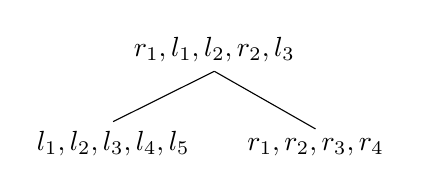
\begin{tikzpicture}[level 1/.style={level distance=1.2cm,sibling distance=0.5cm}]
\Tree [.$r_1,l_1,l_2,r_2,l_3$
$l_1,l_2,l_3,l_4,l_5$
$r_1,r_2,r_3,r_4$ ]
\end{tikzpicture}}
  \caption{Before the \nf{Refresh}.}
\end{subfigure}
\hfill
\begin{subfigure}[b]{.29\textwidth}
  \centering
  \resizebox{\columnwidth}{!}{
  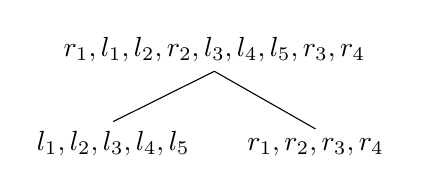
\begin{tikzpicture}[level 1/.style={level distance=1.2cm,sibling distance=0.5cm}]
\Tree [.$r_1,l_1,l_2,r_2,l_3,l_4,l_5,r_3,r_4$
$l_1,l_2,l_3,l_4,l_5$
$r_1,r_2,r_3,r_4$ ]
\end{tikzpicture}}
  \caption{New operations are appended.}
\end{subfigure}
\hspace{6em}
\caption{\label{fig::propagstep} Before and after a \nf{$n$.Refresh} with a successful append. Operations propagating from the left child are labelled with $l$ and from the right child with $r$.}
\end{center}
\end{figure}

\begin{figure}[hbpt]
  \center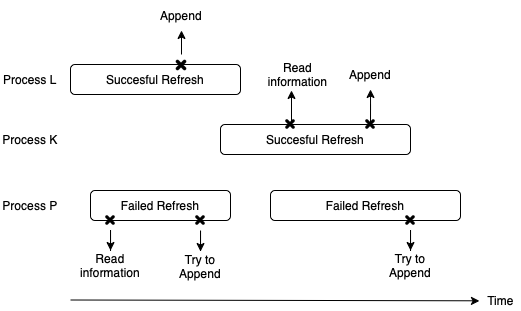
\includegraphics[width=4in]{pics/doublyrefresh.drawio.png}
  \caption{\label{fig::simpleDoubleRefresh}Time relations between the concurrent successful \nf{Refresh}es and the two consecutive \nf{Refresh}es.}
\end{figure}

We use \nf{CAS} (Compare \& Swap) instructions to implement the \nf{Refresh}'s attempt to append  described in the previous paragraph.
The second failed \nf{Refresh} of $P$ is assuredly concurrent with a successful \texttt{Refresh} that has read its information after the invocation of the first failed \nf{Refresh} (see Figure \ref{fig::simpleDoubleRefresh}). This is because some process $L$ does a successful append during $P$'s first failed attempt, and some process $K$ performs a \nf{Refresh} that reads its information after $L$'s append and then performs a successful append during $P$'s second failed \nf{Refresh}. Process $K$'s \nf{Refresh} helps to append the new operations in $n$'s children before $P$'s first failed \nf{Refresh}, in case they were not already appended. After a process appends its operation into its leaf it can call \nf{Refresh} on the path up to the root at most two times on each node. So, with $O(\log p)$ \nf{CAS}es an operation can ensure it appears in the linearization. This cooperative solution allows us to overcome the CAS Retry Problem.


It is not efficient to store the sequence of operations in each node explicitly because each operation would have to be copied all the way up to the root; doing this would not be possible in poly-logarithmic time.
Instead we use an implicit representation of the operations propagated together. Furthermore, we do not need to maintain an ordering on operations propagated together in a node until they have reached the root. It is sufficient to only keep track of sets of operations propagated together in each \nf{Refresh} and then define the linearization ordering only in the root (see Figure \ref{fig::set}). Achieving a constant-sized implicit representation of operations in a \nf{Refresh} allows us to \texttt{CAS} fixed-size objects in each \tt{Refresh}. To do that, we introduce \it{block}s. A block stores information about the operations propagated by a \nf{Refresh}. It contains the number of operations from the left and the right child propagated to the node by the \texttt{Refresh} procedure. See Figure \ref{fig:block} for an example. A node stores an array of blocks of operations propagated up to it. A propagate step  aggregates the new blocks in children into a new block and puts it in the parent's blocks. We call the aggregated blocks \it{subblocks} of the new block and the new block the \it{superblock} of them.  In each \nf{Refresh} there is at most one operation from each process trying to be propagated, because one operation cannot invoke two operations concurrently. Thus, there are at most $p$ operations in a block. Furthermore, since the operations in a \texttt{Refresh} step are concurrent we can linearize them  among themselves in any order we wish, because if two operations are read in one successful \tt{Refresh} step in a node they are going to be propagated up to the root together. Our choice is to put the operations propagated from the left child before the operations propagated from the right child. In this way if we know the number of operations from the left child and the number of operations from the right child in a block  we have a complete ordering on the operations.

\begin{figure}[hbtp]
\begin{center}
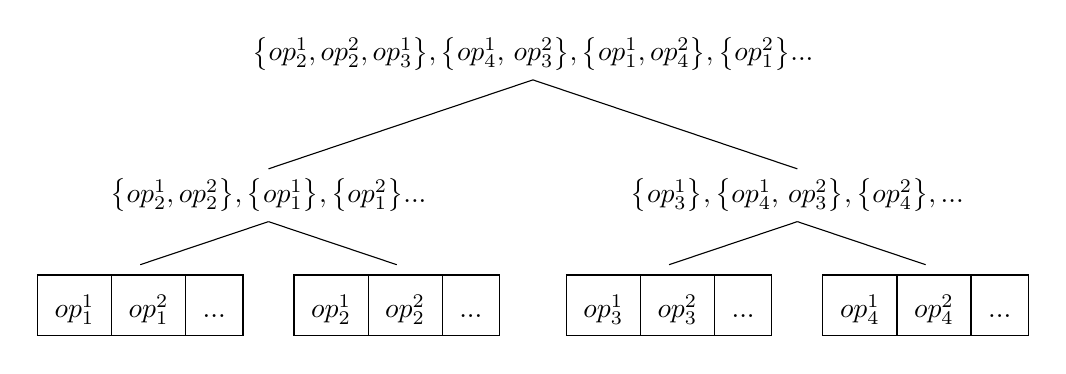
\begin{tikzpicture} [level 1/.style={level distance=1.8cm,sibling distance=0.6cm}, level 2/.style={level distance=1.4cm,sibling distance=0.4cm}]
  
\Tree [.{$\big\{op_2^1,op_2^2,op_3^1\big\},\big\{op_4^1$, $op_3^2\big\},\big\{op_1^1, op_4^2\big\},\big\{op_1^2\big\}...$ }  [.{ $\big\{op_2^1, op_2^2\big\},\big\{op_1^1\big\},\big\{op_1^2\big\}...$ }
      {\begin{tabular}{|l|c|c|c}  \hline $op_1^1$ & $op_1^2$ & ... \\ \hline\end{tabular}} {\begin{tabular}{|l|c|c|c}  \hline $op_2^1$ & $op_2^2$ & ... \\ \hline \end{tabular}} ] [.{ $\big\{op_3^1\big\},\big\{op_4^1$, $op_3^2\big\},\big\{op_4^2\big\},...$ } {\begin{tabular}{|l|c|c|c}  \hline $op_3^1$ & $op_3^2$ & ... \\ \hline\end{tabular}} {\begin{tabular}{|l|c|c|c} \hline $op_4^1$ & $op_4^2$ & ... \\ \hline\end{tabular}} ] ]
\end{tikzpicture}
\caption{\label{fig::set} Leaves are for processes $P_1$ to $P_4$ from left to right. In each internal node one can arbitrarily linearize the sets of concurrent operations  propagated together in a \nf{Refresh}. For example $op_4^1$ and $op_3^2$ have propagated  together in one \nf{Propagate} step and they will be propagated up to the root together. Since their execution time intervals overlap, they can be linearized in any order.}
\end{center}
\end{figure}


\begin{figure}[hbtp]
\begin{center}
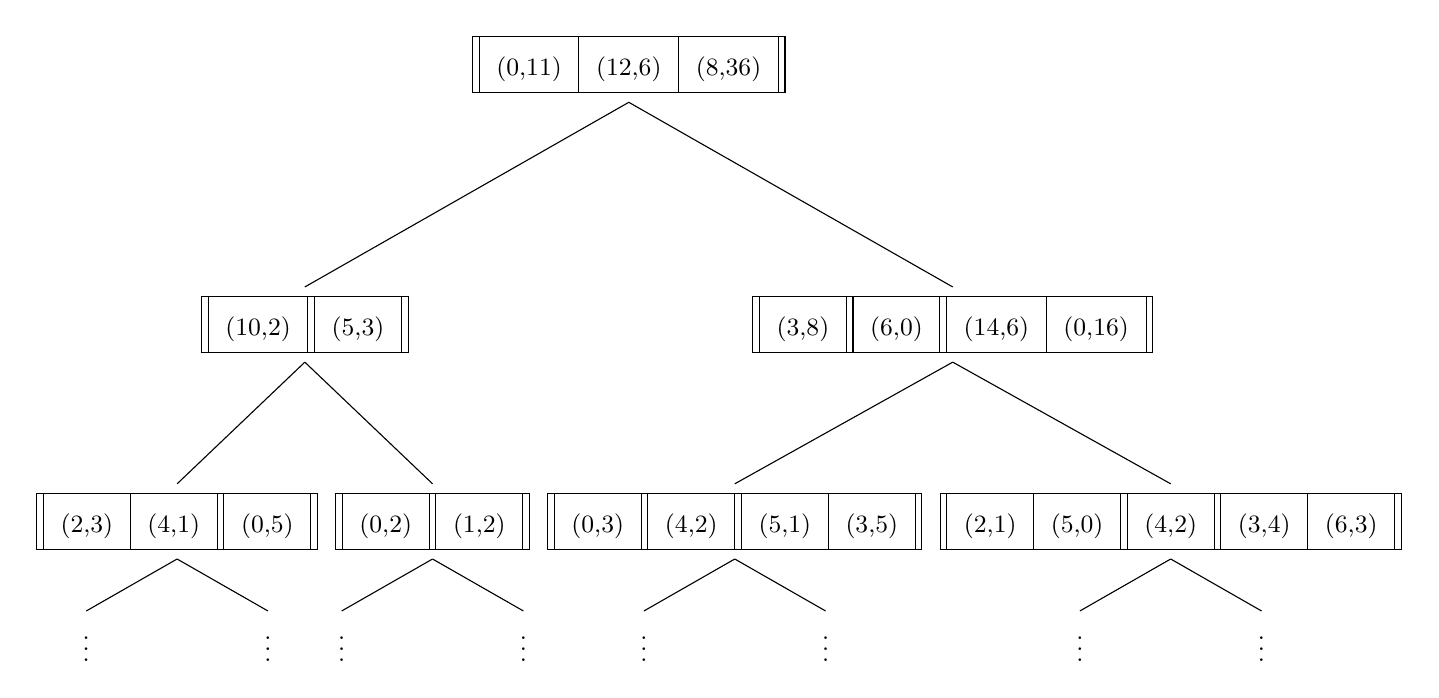
\begin{tikzpicture}
[level 1/.style={level distance=3.3cm,sibling distance=0cm},
	level 2/.style={level distance=2.5cm,sibling distance=0cm},
	level 3/.style={level distance=1.7cm,sibling distance=2cm}]
\begin{small} 

\Tree [.{\begin{tabular}{||c|c|c||}  \hline (0,11) & (12,6) & (8,36) \\ \hline\end{tabular}}
 [.{\begin{tabular}{||c||c||}  \hline (10,2) & (5,3) \\\hline  \end{tabular}}
 [.{\begin{tabular}{||c|c||c||}\hline (2,3) & (4,1) & (0,5) \\\hline\end{tabular}} $\vdots$ $\vdots$ ]
  [.{\begin{tabular}{||c||c||}  \hline (0,2) & (1,2)  \\ \hline  \end{tabular}} $\vdots$ $\vdots$ ] ]
          [.{\begin{tabular}{||c||c||c|c||}  \hline (3,8) & (6,0) & (14,6) & (0,16) \\ \hline \end{tabular}}
           [.{\begin{tabular}{||c||c||c|c||}  \hline (0,3) & (4,2) & (5,1) & (3,5) \\ \hline \end{tabular}} $\vdots$ $\vdots$ ]
            [.{\begin{tabular}{||c|c||c||c|c||}  \hline (2,1) & (5,0) & (4,2) & (3,4) & (6,3) \\ \hline \end{tabular}} $\vdots$ $\vdots$ ] ] ]
\end{small}
\end{tikzpicture}
\end{center}
\caption{\label{fig:block} Using blocks to represent operations. Blocks between two lines $||$ are propagated together to the parent. Each block consists of a pair (left, right) indicating the number of operations from the left and the right child, respectively. For example, (12,6) in the root contains  (10,2) from the left child and (6,0) from the right child. The third block in the root (8,36) is created by merging (5,3) from the left child and (14,6) and (0,16) from the right child. (5,3) is superblock of  (0,5) and (1,2) and (5,1),(3,5) and (4,2) are subblocks of (14,6).}
\end{figure}

So far, we have a shared tree that processes use to agree on the implicit ordering stored in its root. With this agreement on linearization ordering we can design a universal construction; for given object $O$ we can perform an operation $op$ by applying all the operations up until $op$ in the root on a local copy of the object and then returning the response for $op$. However, this approach is not enough for an efficient queue.
We show that we can build an efficien queue if we can compute two things about the ordering in the root: (1) the $i$th propagated operation and (2) the rank of a propagated operation in the linearization. We explain how to implement (1) and (2) in poly-logarithmic steps.

After propagating an operation \texttt{op} to the root, processes can find out information about the linearization ordering using (1) and (2). 
To get the $i$th operation in the root, we find the block $B$ containing the $i$th operation in the root, and then recursively find the subblocks of $B$ in the descendent of the root that contain that $i$th operation. When we reach a block in a leaf, the operation is explicitly stored there. To make this search faster, instead of iterating over all blocks in the node, we store the prefix sum of the number of elements in the blocks sequence to permit a binary search for the required block. We also store pointers to determine the range of subblocks of a block to make the binary search faster. In each block, we store the prefix sum of operations from the left child and from the right child. Moreover, for each block, we store two pointers to the last left and right subblock of it (see Figure \ref{fig::pointer}). We know a block size is at most $p$, so binary search takes at most \textsc{O}$(\log p)$ time, since the pointers of a block and its previous block reduce the search range size to \textsc{O}$(p)$.

To compute the rank in the root of an operation in the leaf, we need to find the superblock of the block that operation is in. After a block is installed in a node we store the approximate index of its superblock in it to make this faster.

\begin{figure}[hbtp]
\centering
  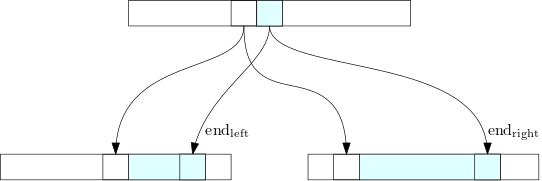
\includegraphics[width=4in, height=1.4in]{pics/pointers}
  \caption{Each block stores the index of its last subblock in each child. \label{fig::pointer}}
\end{figure}

In an execution on a queue where no dequeue operation returns\nf{null}, the $k$th dequeue returns the argument of the $k$th enqueue. In the general case a dequeue returns\nf{null} if and only if the size of the queue after the previous operation is 0. We refer to such a dequeue as a \it{null dequeue}. If the the dequeue is the $k$th non-null dequeue, it returns the argument of the $k$th enqueue. Having the size of the queue after an operation we can compute the number of non-null dequeues from the number of enqueues up to block B. So, if we store the size of the queue after each block of operations in the root, we can compute the index of the enqueue whose argument is the response to a given dequeue in constant time.

In our case of implementing a queue, a process only needs to compute the rank of a \nf{Dequeue} and get an \nf{Enqueue} with a specific rank.  We know we can linearize operations in a block in any order; here, we choose to put \nf{Enqueue} operations in a block before \nf{Dequeue} operations. Consider the following operations, where operations in a cell are concurrent.
\begin{table}[hbtp]
\centering
\begin{small}
\begin{tabular}{c|c|c|c}
    \hline \texttt{Deq} & \texttt{Enq(5)}, \texttt{Enq(2)}, \texttt{Enq(1)}, \texttt{Deq}& \texttt{Enq(3)}, \texttt{Deq}&  \texttt{Enq(4)}, \texttt{Deq}, \texttt{Deq}, \texttt{Deq}, \texttt{Deq}\\ \hline
  \end{tabular}
\end{small}
\end{table}

\noindent The \texttt{Dequeue} operations return \texttt{null, 5, 2, 1, 3, 4, null} respectively.
Now, we claimed that by knowing the size of the queue, we can compute the rank of the required \texttt{Enqueue} for any non-null \nf{Dequeue}. We apply this approach to blocks; if we store the size of the queue after each block of operations happens, we can compute the index of each \nf{Dequeue}'s result in \textsc{O}$(1)$ steps.

\begin{table}[hbtp]
\centering
\begin{small}
  \begin{tabular}{c|c|c|c|c}
    \hline &\texttt{Deq} & \texttt{Enq(5)}, \texttt{Enq(2)}, \texttt{Enq(1)}, \texttt{Deq}& \texttt{Enq(3)}, \texttt{Deq}&  \texttt{Enq(4)}, \texttt{Deq}, \texttt{Deq}, \texttt{Deq}, \texttt{Deq}\\ \hline
    \#\tt{Enq}s & 0 & 3 & 1 & 1 \\ \hline
    \#\tt{Deq}s & 1 & 1 & 1 & 4 \\ \hline
    Size at end & 0 & 2 & 2 & 0 \\ \hline
  \end{tabular}
\end{small}
  \caption{Augmented history of operation blocks on the queue.}
\end{table}

\noindent The size of the queue after the $b$th block in the root could be computed as
$$\textrm{max}\Big(\textrm{size after }b-1\textrm{th block} + \#\textrm{\tt{Enqueue}s in }b\textrm{th block} - \#\textrm{\tt{Dequeue}s in }b\textrm{th block}, 0\Big).$$
\noindent Moreover, the total number of non-null dequeues in blocks $1,2,...,b$ in the root is
$$ \sum_{i=1}^{b} \#\textrm{\tt{Enqueue}s in }i\textrm{th block} - \textrm{size after }b\textrm{th block}.$$

Given a \texttt{Dequeue} is in block $B$, its response is the argument of the \tt{Enqueue} whose rank is the number of non-null \nf{Dequeue}s in  blocks $1,2,...,b-1 + $ index of the \nf{Dequeue} in $B$\textrm{'s} \nf{Dequeue}s, if $\big ($size of the queue after $b-1\textrm{th block} + \#\textrm{\tt{Enqueue}s in }b\textrm{th block} - \#\textrm{index of \tt{Dequeue} in }B\textrm{'s \tt{Dequeue}s} \big )\geq 0$. Otherwise the response would be \nf{null}.


\subsection{Details of the Implementation}
Pseudocode for the queue implementation is given in Section \ref{algQ}. It uses the following two types of objects.
\paragraph{\tt{Node}} 
 In each \texttt{Node} we store pointers to its parent and children, an array of \nf{Block}s called \texttt{block}s and the index \nf{head} of the first empty entry in \texttt{blocks}.

\paragraph{\tt{Block}}
 The information stored in a \nf{Block} depends on whether  the \nf{Block} is in an internal node or a leaf. If it is in a leaf, we use a \nf{LeafBlock} which simply stores one operation. If a block $B$ is in an internal node $n$, then it contains subblocks in the left and right children of $n$. The left subblocks of $B$ are some consecutive blocks in the left child of $n$ starting from where the block prior to $B$ ended. In each \texttt{block} we store four essential fields that implicitly summarize which operations are in the block \texttt{sum\textsubscript{enq-left}}, \texttt{sum\textsubscript{deq-left}}, \texttt{sum\textsubscript{enq-right}}, \texttt{sum\textsubscript{deq-right}}. The \texttt{sum\textsubscript{enq-left}} field is the total number of \nf{Enqueue} operations in the blocks before the last subblock of $B$ in the left child. The other fields' semantics are similar. The \nf{end\sub{left}} and \nf{end\sub{right}} field store the last subblock of a block in the left and the right child, respectively. The approximate index of the superblock of non-root blocks is stored in their \nf{super} field. The \texttt{size} field in a block in the root node stores the size of the queue after the operations in the block have been performed. 

\paragraph{\tt{Enqueue($e$)}}
An \nf{Enqueue} operation does not return a response, so it is sufficient to just propagate the \nf{Enqueue} operation to the root and then use its position in the linearization for future \nf{Dequeue} operations. \nf{Enqueue($e$)} creates a \nf{LeafBlock} with $\nf{element}=e$, sets its \nf{sum\sub{enq}} and \nf{sum\sub{deq}} fields and then appends it to the tree.

\paragraph{\tt{Dequeue()}}
\nf{Dequeue} creates a \nf{LeafBlock}, sets its \nf{sum\sub{enq}} and \nf{sum\sub{deq}} fields and appends it to the tree. Then, it computes the position of the appended \nf{Dequeue} operation in the root using \nf{IndexDequeue} and after that finds the response of the \nf{Dequeue} by calling \nf{FindResponse}.

\paragraph{\tt{FindResponse($b, i$)}}
To compute the response of the $i$th \nf{Dequeue} in the $b$th block of the root Line \ref{checkEmpty} computes whether the queue is empty or not. If there are more \nf{Dequeue}s than \nf{Enqueue}s the queue would become empty before the requested \nf{Dequeue}. If the queue is not empty, Line \ref{computeE} computes the rank $e$ of the \nf{Enqueue} whose argument is response to the \nf{Dequeue}. Knowing the response is the $e$th \nf{Enqueue} in the root (which is before the $b$th block) we find the block and position containing the \nf{Enqueue} operation using \nf{DSearch} and after that \nf{GetEnqueue} finds its \nf{element}.

\paragraph{\tt{Append($B$)}}
The \nf{head} field is the index of the first empty slot in \nf{blocks} in a \nf{LeafBlock}. There are no multiple write accesses on \nf{head} and \nf{blocks} in a leaf because only the process that the leaf belongs to appends to it. \nf{Append($B$)} adds $B$ to the end of the \nf{blocks} field in the leaf, increments \nf{head} and then calls \nf{Propagate} on the leaf's \nf{parent}. When \nf{Propagate} terminates it is guaranteed that the appended block is a subblock of a block in the \nf{root}. 

\paragraph{\tt{Propagate()}}
\nf{Propagate} on node $n$ uses the double refresh idea described in Section \ref{DescriptQ} and invokes two \nf{Refresh}es on $n$ in Lines \ref{firstRefresh} and \ref{secondRefresh}. Then, it invokes \nf{Propagate} on \nf{$n$.parent} recursively until it reaches the root. 

\paragraph{\tt{Refresh()}}
The goal of a \nf{Refresh} on node $n$ is to create a block of $n$'s children's new blocks and append it to $n$\nf{.blocks}. The variable \nf{h} is read from $n$\nf{.head} at Line \ref{readHead}. The new block created by \nf{Refresh} will be inserted into $n\nf{.blocks[h]}$. Lines \ref{startHelpChild1}--\ref{endHelpChild1} of \nf{$n$.Refresh} help to \nf{Advance} $n$'s children. \nf{Advance} increments the children's \nf{head} if necessary and sets the \nf{super} field of their most recent appended blocks. The reason behind this helping is explained later when we discuss \nf{IndexDequeue}. After helping to \nf{Advance} the children, a new block called \nf{new} is created in Line \ref{invokeCreateBlock}. Then, if \nf{new} is empty, \nf{Refresh} returns \nf{true} because there are no new operations to propagate and it is unnecessary to add an empty block to the tree. Later we will use the fact that all blocks contain at least one operation. Line \ref{cas} tries to install \nf{new}. If it was successful all is good. If not, it means someone else has already put a block in $n$\nf{.blocks[h]}. In this case, \nf{Refresh} helps advance $n$\nf{.head} to \nf{h+1} and update the \nf{super} field of $n$\nf{.blocks[h]} at Line \ref{advance}.


\paragraph{\tt{CreateBlock()}} \texttt{$n$.CreateBlock($h$)} is used by \nf{Refresh} to construct a block containing new operations of $n$'s children.
The block \nf{new} is created in Line 333 and its fields are filled similarly for both left and right directions. The variable  \nf{index\sub{prev}} is the index of the block preceding the first subblock in the child in direction \nf{dir} that is aggregated into \nf{new}. Field \texttt{new.end\textsubscript{dir}} stores the index of the rightmost subblock of \nf{new} in the child. Then \nf{sum\sub{enq-dir}} is computed from sum of the the number of \nf{Enqueue} operations in the \nf{new} block from direction \nf{dir} and the value stored in \texttt{$n$.blocks[h-1].sum\sub{enq-dir}}. The field \nf{sum\sub{deq-dir}} is computed similarly. Then, if \nf{new} is going to be installed in the \nf{root}, the \nf{size} field is also computed.

\paragraph{\tt{GetEnqueue($b,i$)} and \tt{DSearch($e, end$)}}
We can describe an operation in a node in two ways: the rank of the operation among all the operations in the node or the index of the block containing the operation in the node and the rank of the operation within that block. If we know the block and rank within the block of an operation we can find the subblock containing the operation and the operation's rank within that subblock in poly-log time. To find the response of a \nf{Dequeue}, we know about the  rank of the response \nf{Enqueue} in the root (\nf{e} in Line \ref{computeE}).
We also know the \nf{e}th \nf{Enqueue} is in \nf{root.blocks[1..end]}. \nf{DSearch} uses doubling to find the range that contains the answer block (Lines \ref{dsearchStart}--\ref{dsearchEnd}) and then tries to find the required indices with a binary search (Line \ref{dsearchBinarySearch}).
A call to \nf{$n$.GetEnqueue($b,i$)} returns the \nf{element} of the $i$th enqueue in $b$th the block of $n$. The range of subblocks of a block is determined using the \nf{end\sub{left}} and \nf{end\sub{right}} fields of the block and its previous block. Then, the subblock is found using binary search on the \nf{sum\sub{enq}} field (Lines \ref{leftChildGet} and \ref{rightChildGet}).

\paragraph{\tt{IndexDequeue($b,i$)}}

A call to $n$\nf{.IndexDequeue($b,i$)} computes the block and the rank within the block in the root of the $i$th \nf{Dequeue} of the $b$th block of $n$. Let $R_n$ be the successful  \nf{Refresh} on node $n$ that did a successful \nf{CAS(null, $B$)} into \nf{n.blocks[$b$]}. Let $par$ be $n$\nf{.parent}. Without loss of generality assume for the rest of this section a ${n}$ is the left child of $par$. Let $R_{par}$ be the first successful \nf{$par$.Refresh} that reads some value greater than ${b}$ for \nf{left.head} and therefore contains ${B}$ in its created block in Line \ref{invokeCreateBlock}. Let $j$ be the index of the block that $R_{par}$ put in $par$\nf{.blocks}.
 
Since the index of the superblock of ${B}$ is not known until $B$ is propagated, $R_n$ cannot set the \nf{super} field of ${B}$ while creating it. One approach for $R_{par}$ is to set the \nf{super} field of ${B}$ after propagating $B$ to $par$. This solution would not be efficient because there might be up to $p$ subblocks in the block $R_{par}$ propagated needing updates their \nf{super} field. However, intuitively, once $B$ is installed, its superblock is going to be close to \nf{$n$.parent.head} at the time of installation. If we know the approximate position of the superblock of $B$ then we can search for the real superblock when it is needed. Thus, \nf{$B$.super} does not have to be the exact location of  the superblock of $B$, but we want it to be close to $j$. We can set \nf{$B$.super} to \nf{$par$.head} while creating $B$, but the problem is that there might be many \nf{Refresh}es on $par$ that could happen after $R_n$ reads $par$\nf{.head} and before propagating $B$ to $par$. If $R_n$ sets \nf{$B$.super} to \nf{$par$.head} after appending $B$ to \nf{$n$.blocks} (Line \ref{setSuper1}), $R_n$ might go to sleep at some time after installing $B$ and before setting \nf{$B$.super}. In this case, the next \nf{Refresh}es on $n$ and $par$ help fill in the value of \nf{$B$.super}.

Block $B$ is appended to \nf{$n$.blocks[$b$]} on Line \ref{cas}. After appending $B$, \nf{$B$.super} is set on Line \ref{setSuper1} of a call to \nf{Advance} from \nf{$n$.Refresh} by the same process or another process or by Line \ref{helpAdvance} of a \nf{$n$.parent.Refresh}. We shall show that this is sufficient to ensure that \nf{$B$.super} differs from the index of $B$'s superblock by at most 1.

\pagebreak
\newpage
\newgeometry{left=0.6in,right=0.6in,top=0.6in,bottom=0.8in}

\subsection{Pseudocode} \label{algQ}
\begin{algorithm}
\caption{Tree Fields Description}
\begin{algorithmic}[1]
\setcounter{ALG@line}{100}
\begin{multicols}{2}

\Statex $\diamondsuit$ \tt{\sl{Shared}}
\begin{itemize}
\item \textsf{A binary tree of \tt{Node}s with one \tt{leaf} for each process. \tt{root} is the root \nf{node}.}
\end{itemize}

\Statex $\diamondsuit$ \tt{\sl{Local}}
\begin{itemize}
\item \tt{\sl{Node} leaf:} \sf{ process's leaf in the tree.}
\end{itemize}

\Statex $\blacktriangleright$ \tt{\sl{Node}}
\begin{itemize}
\item \tt{\sl{*Node} left, right, parent} \textsf{: Initialized  when creating the tree.}
\item \tt{\sl{Block[]} blocks} \textsf{: Initially \tt{blocks[0]} contains an empty block with all fields equal to 0.}
\item \tt{\sl{int} \head= 1}\textsf{: \#\tt{block}s in \tt{blocks}. \tt{blocks[0]} is a block with all integer fields equal to zero.}
\end{itemize}

\Statex $\blacktriangleright$ \tt{\sl{Block}} 

\begin{itemize}
  \item \tt{\sl{int} super}
  \textsf{: approximate index of the superblock, read from \tt{parent.head} when appending the block to the node}
\end{itemize}


\Statex $\blacktriangleright$ \tt{\sl{RootBlock} extends \sl{InternalBlock}}
\begin{itemize}
  \item \tt{\sl{int} \size}
  \textsf{: size of the queue after performing all operations in the prefix for this block}
\end{itemize}

\pagebreak

\Statex $\blacktriangleright$ \tt{\sl{InternalBlock} extends \sl{Block}}
\begin{itemize}
    \item \tt{\sl{int} end\sub{left}, end\sub{right}}
  \textsf{:~~indices of the last subblock of the block in the left and right child}
  \item \tt{\sl{int} sum\sub{enq-left}}
  \textsf{: \# enqueues in \tt{left.blocks[1..end\sub{left}]}}
  \item \tt{\sl{int} sum\sub{deq-left}}
  \textsf{: \# dequeues in \tt{left.blocks[1..end\sub{left}]}}
  \item \tt{\sl{int} sum\sub{enq-right}}
  \textsf{: \# enqueues in \tt{right.blocks[1..end\sub{right}]}}
  \item \tt{\sl{int} sum\sub{deq-right}}
  \textsf{: \# dequeues in \tt{right.blocks[1..end\sub{right}]}}
\end{itemize}

\Statex $\blacktriangleright$ \tt{\sl{LeafBlock} extends \sl{Block}}
\begin{itemize}
  \item \tt{\sl{Object} element}
  \textsf{: Each block in a leaf represents a single operation. If the operation is \tt{enqueue(x)} then \tt{element=x}, otherwise \tt{element=null}.}
  
    \item \tt{\sl{int} sum\sub{enq}, sum\sub{deq}}
  \textsf{: \# enqueue, dequeue operations in the prefix for the block}
\end{itemize}

\end{multicols}
\end{algorithmic}
\end{algorithm}

\begin{footnotesize}

\it{Abbreviations used in the code and the proof of correctness.}
\begin{itemize}
 \item \tt{blocks[b].sum\sub{x}=blocks[b].sum\sub{x-left}+blocks[b].sum\sub{x-right}}  \tt{ (for internal blocks where b$\geq$0 and x $\in$ \{enq, deq\}})
%  \item \tt{blocks[b].sum=blocks[b].sum\sub{enq}+blocks[b].sum\sub{deq}}  \tt{ (for b$\geq$0})
  \item \tt{blocks[b].num\sub{x}=blocks[b].sum\sub{x}-blocks[b-1].sum\sub{x}} \\ \tt{(for all blocks where b>0 and x $\in$ \{ enq, deq, enq-left, enq-right, deq-left, deq-right\})}
\end{itemize}
\end{footnotesize}

\pagebreak

\begin{algorithm}
\caption{\tt{\sl{Queue}}}
\begin{algorithmic}[1]
\setcounter{ALG@line}{200}


\Function{void}{Enqueue}{\sl{Object} e} \cmt{Creates a \tt{block} with element \tt{e} and adds it to the tree.}
\State \tt{block newBlock= \Call{new}{\sl{LeafBlock}}}
\State \tt{newBlock.element= e}
\State \tt{newBlock.sum\sub{enq}= leaf.blocks[leaf.\head].sum\sub{enq}+1}
\State \tt{newBlock.sum\sub{deq}= leaf.blocks[leaf.\head].sum\sub{deq}}
\State \tt{leaf.}\Call{Append}{newBlock}
\EndFunction{Enqueue}

\Statex

\Function{Object}{Dequeue()}{} \cmt{Creates a block with\nf{null} value element, appends it to the tree and returns its response.}
\State \tt{block newBlock= \Call{new}{\sl{LeafBlock}}} 
\State \tt{newBlock.element= null}
\State \tt{newBlock.sum\sub{enq}= leaf.blocks[leaf.\head].sum\sub{enq}}
\State \tt{newBlock.sum\sub{deq}= leaf.blocks[leaf.\head].sum\sub{deq}+1}
\State \tt{leaf.}\Call{Append}{newBlock}
\State \tt{<b, i>=} \Call{IndexDequeue}{leaf.\head, 1}
\State \tt{output=} \Call{FindResponse}{b, i} 
\label{deqRest}
\State \Return{\tt{output}}
\EndFunction{Dequeue}

\Statex

\Function{element}{FindResponse}{\sl{int} b, \sl{int} i}\cmt{Returns the response to $D_i(root,b)$, the \nf{i}th \nf{Dequeue} in \nf{root.blocks[b]}.}
\If{\tt{ root.blocks[b-1].\size}\tt{ + root.blocks[b].num\sub{enq} - i $<$ 0}} \label{checkEmpty}\cmt{Check if the queue is empty.}
\State \Return \tt{null} \label{returnNull}
\Else
\State \tt{e= i - root.blocks[b-1].size + root.blocks[b-1].sum\sub{enq}} \label{computeE}
\cmt{The response is $E_e(root)$, the \nf{e}th \nf{Enqueue}in the root.}
\State \Return \tt{root.GetEnqueue(root.\Call{DSearch}{e, b})}\label{findAnswer}
\EndIf
\EndFunction{FindResponse}

\end{algorithmic}
\end{algorithm}

\pagebreak


\begin{algorithm}
\caption{Root}
\begin{algorithmic}[1]
\setcounter{ALG@line}{800}
\Statex
\Statex $\leadsto$ \textsf{Precondition: \tt{root.blocks[end].sum\sub{enq} $\geq$ \tt{e}}}
\Statex $\triangleright$ \textmd{Returns \tt{<b,i>} such that $E_e(root)=E_i(root,b)$,i.e. , the \nf{e}th \nf{Enqueue} in the \nf{root} is the \nf{i}th \nf{Enqueue} within block \nf{b} of the \nf{root}.}

\Function{<int, int>}{DSearch}{\sl{int} e, \sl{int} end}
\State \tt{start= end-1} \label{dsearchStart}
\While{\tt{root.blocks[start].sum\sub{enq}}$\geq$\tt{e}}
\State \tt{start= max(start-(end-start), 0)} \label{doubling}
\EndWhile \label{dsearchEnd}
\State \tt{b= root.BinarySearch( e, start, end)} \label{dsearchBinarySearch}
\State \tt{i= e- root.blocks[b-1].sum\sub{enq}} \label{DSearchComputei}
\State\Return \tt{<b,i>}
\EndFunction{DSearch}
\end{algorithmic}
\end{algorithm}

\begin{algorithm}
\caption{Leaf}
\begin{algorithmic}[1]
\setcounter{ALG@line}{600}

\Function{void}{Append}{\sl{block} B} \cmt{Only called by the owner of the leaf.}
\State \tt{blocks[\head]= B} 
\State \tt{\head+=1} \label{appendEnd} 
\State \tt{parent.}\Call{Propagate()}{} 
\EndFunction{Append}

\end{algorithmic}
\end{algorithm}


\pagebreak

\begin{algorithm}
\caption{\tt{\sl{Node}}}
\begin{algorithmic}[1]
\setcounter{ALG@line}{300}
\begin{multicols}{2}

\Statex $\triangleright$ \textmd{\nf{$n$.Propagate} propagates operations  in \nf{this}.children up to \nf{this} when it terminates.}
\Function{void}{Propagate()}{}
\If{\bf{not} \Call{Refresh()}{}} \label{firstRefresh}
\State \Call{Refresh()}{} \label{secondRefresh}
\EndIf
\If{\tt{this} \bf{is not} \tt{root}}
\State \tt{parent.}\Call{Propagate()}{}
\EndIf
\EndFunction{Propagate}

\Statex

\Statex $\triangleright$ \textmd{Creates a block containig new operations of \nf{this.}children, and then tries to append it to \nf{this}.}
\Function{boolean}{Refresh()}{}
\State \tt{h= \head} \label{readHead}
\ForEach{\tt{dir} {\keywordfont{in}} \tt{\{left, right\}}} \label{startHelpChild1}
\State \tt{h\sub{dir}= dir.\head} \label{readChildHead}
\If{\nf{dir.blocks[h\sub{dir}]!=null}} \label{ifHeadnotNull}
\State{\tt{dir.\Call{Advance}{h\sub{dir}}}} \label{helpAdvance}
\EndIf
\EndFor \label{endHelpChild1}
\State \tt{new= \Call{CreateBlock}{h}} \label{invokeCreateBlock}
\If{\tt{new.num==0}} \Return{\tt{true}} \label{addOP} 
\EndIf
\State{\tt{result= blocks[h].CAS(null, new)}} \label{cas}
\State{\tt{this.\Call{Advance}{h}}} \label{advance}
\State \Return{ \tt{result}}

\EndFunction{Refresh}

\Statex

\Function{void}{Advance}{\sl{int} h}
\State \tt{h\sub{p}= parent.\head} \label{readParentHead}
\State \tt{blocks[h].super.CAS(null, h\sub{p}} \label{setSuper1}
\State \tt{head.CAS(h, h+1)} \label{incrementHead}
\EndFunction{Advance}

\pagebreak
\Statex $\leadsto$ \textsf{Precondition: \tt{blocks[start..end]} contains a block with \tt{sum\sub{enq}} greater than or equal to \tt{i}}
\Statex $\triangleright$ \textmd{Does a binary search for~the value \tt{i} of \tt{sum\sub{enq}} field. Returns the index of the leftmost block in \tt{blocks[start..end]} whose \tt{sum\sub{enq}} is $\geq$ \tt{i}}.
\Function{int}{BinarySearch}{ \sl{int} i, \sl{int} start, \sl{int} end}
\State \Return \tt{min\{j: blocks[j].sum\sub{enq}$\geq$i\}}
\EndFunction{BinarySearch}

\Statex

\Statex\cmt{Creates and returns the block to be installed in \tt{blocks[i]}. Created block includes \tt{left.blocks[index\sub{prev}+1..index\sub{last}]} and \tt{right.blocks[index\sub{prev}+1..index\sub{last}]}.}
\Function{Block}{CreateBlock}{\sl{int} i} 
\State \tt{block new= \Call{new}{\sl{block}}}
\ForEach{\tt{dir} {\keywordfont{in}} \tt{\{left, right\}}}
\State \tt{index\sub{prev}= blocks[i-1].end\sub{dir}} \label{prevLine}
\State \tt{new.end\sub{dir}= dir.\head-1} \label{lastLine}
\State \tt{block\sub{prev}= dir.blocks[index\sub{prev}]}
\State \tt{block\sub{last}= dir.blocks[new.end\sub{dir}]}
\State \tt{new.sum\sub{enq-dir}= blocks[i-1].sum\sub{enq-dir} + }
\Statex \hspace{10.7em}\tt{block\sub{last}.sum\sub{enq} - block\sub{prev}.sum\sub{enq}} \label{setSumEnqLeft}
\State \tt{new.sum\sub{deq-dir}= blocks[i-1].sum\sub{deq-dir} + }
\Statex \hspace{10.7em}\tt{block\sub{last}.sum\sub{deq} - block\sub{prev}.sum\sub{deq}} \label{setSumEnqRight}
\EndFor
\If{\tt{this} \bf{is} \tt{root}}
\State \tt{new.\size= max(root.blocks[i-1].\size { }+ new.num\sub{enq}}
\Statex \hspace{8.5em} \tt{- new.num\sub{deq}, 0)}\label{computeLength}
\EndIf

\State \Return \tt{new}
\EndFunction{CreateBlock}

\end{multicols}
\end{algorithmic}
\end{algorithm}

\pagebreak

\begin{algorithm}
\caption{Node}
\begin{algorithmic}[1]
\setcounter{ALG@line}{400}

\Statex $\leadsto$ \textsf{Precondition:~\tt{blocks[b].num\sub{enq}$\geq$i$\geq 1$}}
\Function{element}{GetEnqueue}{\sl{int} b, \sl{int} i} \cmt{Returns the element of $E_i(this,b)$.}
\If{\tt{this} \bf{is} \tt{leaf}}
\State\Return \tt{blocks[b].element} \label{getBaseCase}
\ElsIf{\tt{i $\leq$ blocks[b].num\sub{enq-left}}} \label{leftOrRight} \cmt{$E_i(this,b)$ is in the left child of this node.}
\State \tt{subBlock= left.\Call{BinarySearch}{ i+blocks[b-1].sum\sub{enq-left}, blocks[b-1].end\sub{left}+1, blocks[b].end\sub{left}}} \label{leftChildGet}
\State \Return\tt{left.}\Call{GetEnqueue}{subBlock, i} 
\Else
\State \tt{i= i-blocks[b].num\sub{enq-left}}
\State\tt{subBlock= right.\Call{BinarySearch}{ i+blocks[b-1].sum\sub{enq-right}, blocks[b-1].end\sub{right}+1, blocks[b].end\sub{right}}} \label{rightChildGet}
\State \Return\tt{right.}\Call{GetEnqueue}{subBlock, i} 
\EndIf
\EndFunction{GetEnqueue}

\Statex
\Statex $\leadsto$ \textsf{Precondition: \tt{b}th block of the node has propagated up to the root and \tt{blocks[b].num\sub{deq}$\geq$i}.}
\Function{<int, int>}{IndexDequeue}{\sl{int} b, \sl{int} i} \cmt{Returns \tt{<x, y>} if $D_i(this, b)=D_y(root,x)$.}
\If{\tt{this} \bf{is} \tt{root}}
\State\Return \tt{<b, i>} \label{indexBaseCase}
\Else
\State \tt{dir= (parent.left==n ? left: right)} 
\State \tt{sb= (parent.blocks[blocks[b].super].sum\sub{deq-dir} > blocks[b].sum\sub{deq} ?  blocks[b].super: blocks[b].super+1)}\label{computeSuper}

\If{\tt{dir {\keywordfont is} left}} \label{computeISuperStart}
\State \tt{i+= blocks[b-1].sum\sub{deq}-parent.blocks[sb-1].sum\sub{deq-left}} \label{considerPreviousLeft}
\Else \label{considerRight}
\State \tt{i+= blocks[b-1].sum\sub{deq}-parent.blocks[sb-1].sum\sub{deq-right}}  \label{considerPreviousRight}
\State \tt{i+= parent.blocks[sb].num\sub{deq-left}}  \label{considerLeftBeforeRight}
\EndIf \label{computeISuperEnd}
\State \Return\tt{this.parent.}\Call{IndexDequeue}{sb, i}
\EndIf
\EndFunction{IndexDequeue}

\end{algorithmic}
\end{algorithm}

\restoregeometry
\newpage
\clearpage

\section{Proof of Correctness}

We adopt linearizability as our definition of correctness. In our case, where we create the linearization ordering in the root, we need to prove (1) the ordering is legal, i.e, for every execution on our queue if operation $op_1$ terminates before operation $op_2$ then $op_1$ is linearized before operation $op_2$ and (2) if we do operations sequentially in their the linearization order, operations get the same results as in our queue. The proof is structured like this. First, we define and prove some facts about blocks and the node's \nf{head} field. Then, we introduce  the linearization ordering formally. Next, we prove double \nf{Refresh} on a node is enough to propagate its children's new operations up to the node, which is used to prove (1). After this, we prove some claims about the size and operations of each block, which we use to prove the correctness of \nf{DSearch()}, \nf{GetEnqueue()} and \nf{IndexDequeue()}. Finally, we prove the correctness of the way we compute the response of a dequeue, which establishes (2).

\subsection{Basic Properties}
In this subsection we talk about some properties of blocks and fields of the tree nodes.

A block is an object storing some statistics, as described in Algorithm Queue. A block in a node implicitly represents a set of operations.
\begin{definition}[Ordering of a block in a node]
Let $b$ be \nf{$n$.blocks[$i$]} and $b^\prime$ be \nf{$n$.blocks[$j$]}. We call $i$ the \emph{index} of block $b$. Block $b$ is \it{before} block $b^\prime$ in node $n$ if and only if $i<j$. We define \it{the prefix for} block $b$ in node $n$ to be the blocks in \tt{$n$.blocks[0..$i$]}.
\end{definition}

Next, we show that the value of \nf{head} in a node can only be increased. By the termination of a \nf{Refresh}, \nf{head} has been incremented by the process doing the \nf{Refresh} or by another process.
\begin{observation} \label{nonDecreasingHead}
For each node $n$,  $n.\nf{head}$ is non-decreasing over time.
\end{observation}
\begin{proof}
  The claim follows trivially from the code since \nf{head} is only changed by incrementing in Line \ref{incrementHead} of \nf{Advance}.
\end{proof}

\begin{lemma} \label{lem::headInc}
Let $R$ be an instance of \nf{Refresh} on a node $n$. After $R$ terminates, \nf{$n$.head} is greater than the value read in line \ref{readHead} of $R$.
\end{lemma}
\begin{proof}
If the \nf{CAS} in Line \ref{incrementHead} is successful then the claim holds. Otherwise $n.\nf{head}$ has changed from the value that was read in Line \ref{readHead}. By Observation \ref{nonDecreasingHead} this means another process has incremented $n.\nf{head}$.
\end{proof}

Now we show \nf{$n$.blocks[$n$.head]} is either the last block written into node $n$ or the first empty block in~$n$.

\begin{invariant}[headPosition] \label{lem::headPosition} If the value of $n.\nf{head}$ is $h$ then $\nf{$n$.blocks[$i$]}=\nf{null}$ for ${i>h}$ and $\nf{$n$.blocks[$i$]}\neq\nf{null}$ for ${0\leq i<h}$.
\end{invariant}
\begin{proof}
Initially the invariant is true since $n.\nf{head}=1$, $n.\nf{blocks[0]}\neq\nf{null}$  and $n.\nf{blocks[$x$]}=\nf{null}$ for every $x>0$. The truth of the invariant may be affected by writing into \nf{n.blocks} or incrementing \nf{n.head}. We show that if the invariant holds before such a change  then it  still holds after the change.

In the algorithm, $n.\nf{blocks}$ is modified only on Line \ref{cas}, which updates $n.\nf{blocks[$h$]}$ where $h$ is the value read from $n.\nf{head}$ in Line \ref{readHead}. Since the \nf{CAS} in Line \ref{cas} is successful it means $n.\nf{head}$ has not changed from $h$ before doing the \nf{CAS}: if $n$\nf{.head} had changed before the \nf{CAS} then it would be greater than $h$ by Observation \ref{nonDecreasingHead} and hence $n$\nf{.blocks[}$h$\nf{]}$\neq$\nf{null} and by the induction hypothesis, so the \nf{CAS} would fail. Writing into \nf{$n$.blocks[$h$]} when $h=n$\nf{.head} preserves the invariant, since the claim does not talk about the content of \nf{$n$.blocks[$n$.head]}.

The value of \nf{n.head} is modified only in Line \ref{incrementHead} of \nf{Advance}. If $n$\nf{.head} is incremented to $h+1$ it is sufficient to show \nf{n.blocks[$h$]}$\neq$\nf{null}. \nf{Advance} is called  in Lines \ref{helpAdvance} and \ref{advance}. For Line \ref{helpAdvance}, $n.\nf{blocks[h]}\neq\nf{null}$ because of the \nf{if} condition in Line \ref{ifHeadnotNull}. For Line \ref{advance}, Line \ref{cas} was finished  before doing \ref{advance}. Whether Line \ref{cas} is successful or not, $n.\nf{blocks[h]}\neq\nf{null}$ after the $n$\nf{.blocks[$h$].CAS}. 
\end{proof}

We define the subblocks of a block recursively.

\begin{definition}[Subblock]\label{def::subblock}
A block is a \emph{direct subblock} of the $i$th block in node $n$ if it is\\ in $$\texttt{$n$.left.blocks[$n$.blocks[$i-1$].end\textsubscript{left}+1$\cdots n$.blocks[$i$].end\textsubscript{left}]}$$ or in $$\texttt{$n$.right.blocks[$n$.blocks[$i-1$].end\textsubscript{right}+1$\cdots n$.blocks[$i$].end\textsubscript{right}]}.$$ Block $b$ is a \emph{subblock} of block $c$ if $b$ is a direct subblock of $c$ or a subblock of a direct subblock of $c$.  We say block $b$ is \it{propagated} to node $n$ if $b$ is in $n.blocks$ or is a subblock of a block in $n\nf{.blocks}$.
\end{definition}

The next lemma is used to prove the subblocks of two blocks in a node are disjoint.
\begin{lemma} \label{lem::headProgress}
 If $n\nf{.blocks[}i\nf{]}\neq\nf{null}$ and $i>0$ then $\nf{$n$.blocks[$i$].end\sub{left}} \geq \nf{$n$.blocks[$i-1$].end\sub{left}}$ and $\nf{$n$.blocks[$i$].end\sub{right}} \geq \nf{$n$.blocks[$i-1$].end\sub{right}}$.
\end{lemma}
\begin{proof}
Consider the block $b$ written into \nf{n.blocks[$i$]} by \nf{CAS} at Line \ref{cas}. Block $b$ is created by the \nf{CreateBlock($i$)} called at Line \ref{invokeCreateBlock}. Prior to this call to \nf{CreateBlock($i$)}, $\nf{n.head}=i$ at Line \ref{readHead}, so \nf{n.blocks[$i-1$]} is already a non-null value $b$$^\prime$ by Invariant \ref{lem::headPosition}. Thus, the \nf{CreateBlock($i-1$)} that created  $b^\prime$ terminated before the \nf{CreateBlock($i$)} that creates $b$ is invoked. The value written into \nf{$b$.end\sub{left}} at Line \ref{lastLine} of \nf{CreateBlock($i$)}  was one less than the value read at Line \ref{lastLine} of \nf{CreateBlock($i$)}. Similarly, the value in \nf{n.blocks[$i-1$].end\sub{left}} was one less than the value read from $\nf{n.left.head}$ during the call to \nf{CreateBlock($i-1$)}. By Observation \ref{nonDecreasingHead}, $n\nf{.left.head}$ is non-decreasing, so $b^\prime\nf{.end\sub{left}} \leq \nf{$b$.end\sub{left}}$. The proof for \nf{end\sub{right}} is similar.
\end{proof}

\begin{lemma} \label{lem::subblocksDistinct}
Subblocks of any two blocks in node $n$ do not overlap.  
\end{lemma}
\begin{proof}
We are going to prove the lemma by contradiction. Consider the lowest \nf{node} $n$ in the tree that violates the claim. Then subblocks of $n\nf{.blocks[}i\nf{]}$ and $n\nf{.blocks[}j\nf{]}$ overlap for some $i<j$. Since $n$ is the lowest node in the tree violating the claim, direct subblocks of blocks of $n\nf{.blocks[}i\nf{]}$ and $n\nf{.blocks[}j\nf{]}$ have to overlap. Without loss of generality assume left child subblocks of $n\nf{.blocks[}i\nf{]}$ overlap with the left child subblocks of $n\nf{.blocks[}j\nf{]}$. By Lemma \ref{lem::headProgress} we have $ \nf{$n$.blocks[$i$].end\sub{left}} \leq \nf{$n$.blocks[$j-1$].end\sub{left}}$, so the ranges $[\nf{$n$.blocks[$i-1$].end\sub{left}}+1 \cdots \nf{$n$.blocks[$i$].end\sub{left}}]$ and $[\nf{$n$.blocks[$j-1$].end\sub{left}}+1 \cdots \nf{$n$.blocks[$j$].end\sub{left}}]$ cannot overlap. Therefore, direct subblocks of \nf{$n$.blocks[$i$]} and \nf{$n$.blocks[$j$]} cannot overlap.
\end{proof}

\begin{definition}[Superblock]
  Block $b$ is \it{superblock} of block $c$ if $c$ is a direct subblock of $b$.
\end{definition}
\begin{corollary}
Every block has at most one superblock.
\end{corollary}
\begin{proof}
A block having more than one superblock contradicts Lemma \ref{lem::subblocksDistinct}.
\end{proof}

Now we can define the operations of a block using the definition of subblocks.
\begin{definition}[Operations of a block]\label{def::ops}
A block $b$ in a leaf represents an \nf{Enqueue} if $b\nf{.element}\neq\nf{null}$. Otherwise, if $b\nf{.element}=\nf{null}$, $b$ represents a \nf{Dequeue}. The set of operations of block $b$ is the union of the operations in leaf subblocks of $b$. We denote the set of operations of block $b$ by ${ops(b)}$ and the union  of operations of a set of blocks $B$ by $ops(B)$.  We also say ${b}$ contains ${op}$ if $op\in{ops(b)}$.
\end{definition}

Operations are distinct \nf{Enqueue}s and \nf{Dequeue}s invoked by processes. The next lemma proves that each operation appears at most once in the blocks of a node.
\begin{lemma}\label{lem::noDuplicates}
If $op$ is in $n.blocks[i]$ then there is no $j\neq i$ such that $op$ is in $n.blocks[j]$.
\end{lemma}
\begin{proof}
We prove this claim using Lemma \ref{lem::subblocksDistinct}. Assume $op$ is in the subblocks of both $n.blocks[i]$ and $n.blocks[j]$. From Corollary \ref{lem::subblocksDistinct} we know that the subblocks of these blocks are different, so there are two leaf blocks containing $op$. Since each process puts each operation in only one block of its leaf then $op$ cannot be in two leaf blocks. This is a contradiction.
\end{proof}

\begin{definition}
$n\nf{.blocks[}i\nf{]}$ is \emph{established} at time $t$ if $n\nf{.head}>i$. An operation is \it{established} in node $n$ if it is in an established block of $n$. $EST^n_t$ is the set of established operations in node $n$ at time $t$.
\end{definition}

Now we want to say the blocks of a node grow over time.
\begin{observation}\label{lem::blocksOrder}
  If  time $t<$ time $t^\prime$ ($t$ is before $t^\prime$), then $ops(n.blocks)$ at time $t$ is a subset of $ops(n.blocks)$ at time $t^\prime$.
\end{observation}
\begin{proof}
Blocks are only appended (not modified) with \nf{CAS} to $n\nf{.blocks[}n\nf{.head]}$, so the set of blocks of a node after the \nf{CAS} contains the the set of blocks before the \nf{CAS}.
\end{proof}

\begin{corollary}\label{lem::establishedOrder}
  If  time $t<$ time $t^\prime$, then $EST_n^t\subseteq EST_n^{t^\prime}$.
\end{corollary}
\begin{proof}
From Observations \ref{nonDecreasingHead}, \ref{lem::blocksOrder}.  
\end{proof}

\pagebreak

\subsection{Ordering Operations}

\begin{figure}[hbt]
  \center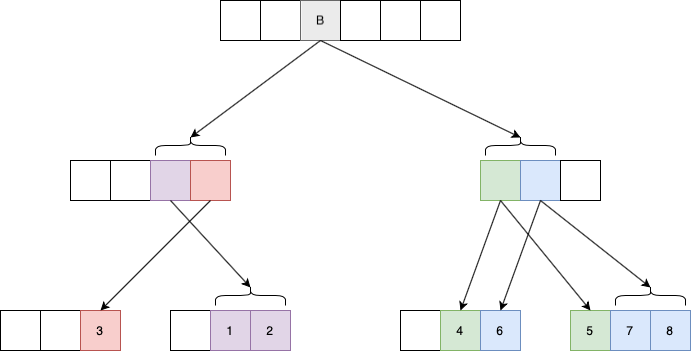
\includegraphics[width=5.5in]{pics/tree}
  \caption{Order of operations in b. Operations in the leaves are ordered with numerical order shown in the drawing.}
\end{figure}

Now we define the ordering of operations stored in each node. In the non-root nodes we only need to order operations of a type among themselves. Processes are numbered from 1 to $p$ and leaves of the tree are assigned from left to right. We will show in Lemma \ref{blockSize} that there is at most one operation from each process in a given block.
\begin{definition} [Ordering of operations inside the nodes] \label{ordering}
\end{definition}
\begin{itemize}
  \item $E(n,b)$ is the sequence of enqueue operations in $ops(n\nf{.blocks[}b\nf{]})$ defined recursively as follows. $E(leaf,b)$ is the single enqueue operation in $ops(leaf\nf{.blocks[}b\nf{]})$ or an empty sequence if $leaf\nf{.blocks[}b\nf{]}$ represents a dequeue operation. If $n$ is an internal node, then
\begin{align*} 
E(n,b) =&  E(n\nf{.left},n\nf{.blocks[}b-1\nf{].end\sub{left}}+1)\cdots E(n\nf{.left},n\nf{.blocks[}b\nf{].end\sub{left}})\cdot \\ 
&E(n\nf{.right},n\nf{.blocks[}b-1\nf{].end\sub{right}}+1)\cdots E(n\nf{.right},n\nf{.blocks[}b\nf{].end\sub{right}}).
\end{align*}
  \item $E_i(n,b)$ is the $i$th enqueue in $E(n,b)$.
\item The order of the enqueue operations in the node $n$ is $E(n)=E(n,1)\cdot E(n,2)\cdot E(n,3)\cdots$
\item $E_i(n)$ is the $i$th enqueue in $E(n)$.
  \item $D(n,b)$ is the sequence of dequeue operations in $ops(n\nf{.blocks[}b\nf{]})$ defined recursively as follows. $D(leaf,b)$ is the single dequeue operation in $ops(leaf\nf{.blocks[}b\nf{]})$ or an empty sequence if $leaf\nf{.blocks[}b\nf{]}$ represents an enqueue operation. If $n$ is an internal node, then
\begin{align*} 
D(n,b) =&  D(n\nf{.left},n\nf{.blocks[}b-1\nf{].end\sub{left}}+1)\cdots D(n\nf{.left}, n\nf{.blocks[}b\nf{].end\sub{left}})\cdot \\ 
&D(n\nf{.right},n\nf{.blocks[}b-1\nf{].end\sub{right}}+1)\cdots D(n\nf{.right},n\nf{.blocks[}b\nf{].end\sub{right}}).
\end{align*}
    \item $D_i(n,b)$ is the $i$th enqueue in $D(n,b)$.
\item The order of the dequeue operations in the node $n$ is $D(n)=D(n,1)\cdot D(n,2)\cdot D(n,3)...$
\item $D_i(n)$ is the $i$th dequeue in $D(n)$.
\end{itemize}

The linearization ordering is given by the order that operations appear in the blocks in the root.
\begin{definition}[Linearization] \label{def::lin}
 $$L=E(root,1)\cdot D(root,1)\cdot E(root,2)\cdot D(root,2)\cdot E(root,3)\cdot D(root,3)\cdots$$
\end{definition}

\begin{observation}\label{sumToNum}
For any node $n$ and indices $i<j$ of \nf{blocks} in $in$, we have
$$n.\nf{blocks[}j\nf{].sum\sub{x}}-n.\nf{blocks[}i\nf{].sum\sub{x}}=\mathlarger{\sum}_{k=i+1}^{j}  n\nf{.blocks[}k\nf{].num\sub{x}}$$ where \nf{x} in $\{\nf{enq}, \nf{deq}, \nf{enq-left}, \nf{enq-right}, \nf{deq-left}, \nf{deq-right}\}$.
\end{observation}

Next claim is also true if we replace \nf{enq} with \nf{deq} and $E$ with $D$.
\begin{lemma}\label{lem::numX}
Let $B$, $B^\prime$ be $n\nf{.blocks[}b\nf{]}$, $n\nf{.blocks[}b-1\nf{]}$ respectively.
\begin{enumerate}[label=(\arabic*)]
    \item If $n$ is an internal node $B\nf{.num\sub{enq-left}}=\Big|E(n.\nf{left},B^\prime.\nf{end\sub{left}}+1)\cdots E(n.\nf{left},B.\nf{end\sub{left}})\Big|$.
    \item If $n$ is an internal node $B\nf{.num\sub{enq-right}}=\Big|E(n.\nf{right},B^\prime.\nf{end\sub{right}}+1)\cdots E(n.\nf{right},B.\nf{end\sub{right}})\Big|$.
    \item $B\nf{.num\sub{enq}}=\Big|E(n,b)\Big|$.
\end{enumerate}
\end{lemma}
\begin{proof}
 We prove the claim by induction on height of node $n$. Base case (3) for leaves is trivial. Supposing the claim is true for $n$'s children, we prove the correctness of the claim for $n$.
\begin{align*}
    B\nf{.num\sub{enq-left}}=&B.\nf{sum\sub{enq-left}}-B^\prime.\nf{sum\sub{enq-left}}& \text{Definition of }\nf{num\sub{enq}}\\
    =& B^\prime.\nf{sum\sub{enq-left}}+n\nf{.left.blocks[}B\nf{.end\sub{left}].sum\sub{enq}}\\&-n\nf{.left.blocks[}B^\prime\nf{.end\sub{left}].sum\sub{enq}}-B^\prime.\nf{sum\sub{enq-left}} & \nf{CreateBlock}\\
    =& n.\nf{left.blocks[}B\nf{.end\sub{left}].sum\sub{enq}}- n.\nf{left.blocks[}B^\prime\nf{.end\sub{left}].sum\sub{enq}}\\
    =& \sum_{i=B^\prime\nf{.end\sub{left}}+1}^{B\nf{.end\sub{left}}}  n\nf{.left.blocks[}i\nf{].num\sub{enq}} &\text{Observation } \ref{sumToNum}\\
    =& \Big|E(n.\nf{left},B^\prime.\nf{end\sub{left}}+1)\cdots E(n.\nf{left},B.\nf{end\sub{left}})\Big| & \textrm{Induction hypothesis (3)}
\end{align*}
The last line holds because of the induction hypothesis (3). (2) is similar to (1). Now we prove (3) starting from the Definition of $E(n,b)$.
\begin{align*} 
E(n,b) =&  E(n\nf{.left},n\nf{.blocks[}b-1\nf{].end\sub{left}}+1)\cdots E(n\nf{.left},n\nf{.blocks[}b\nf{].end\sub{left}})\cdot \\ 
&E(n\nf{.right},n\nf{.blocks[}b-1\nf{].end\sub{right}}+1)\cdots E(n\nf{.right},n\nf{.blocks[}b\nf{].end\sub{right}}).
\end{align*}
By (1) and (2) we have $\Big|E(n,b)\Big|=B\nf{.num\sub{enq-left}}+B\nf{.num\sub{enq-right}}=B\nf{.num\sub{enq}}$.
\end{proof}

Next claim is also true if we replace \nf{enq} with \nf{deq} and $E$ with $D$.
\begin{corollary}\label{lem::sumX}
Let $B$ be $n\nf{.blocks[}b\nf{]}$ and \nf{enq} be in $\{\nf{enq},\nf{deq}\}$.
\begin{enumerate}[label=(\arabic*)]
    \item If $n$ is an internal node $B\nf{.sum\sub{enq-left}}=\Big|E(n.\nf{left},1)\cdots E(n.\nf{left},B.\nf{end\sub{left}})\Big|$
    \item If $n$ is an internal node $B\nf{.sum\sub{enq-right}}=\Big|E(n.\nf{right},1)\cdots E(n.\nf{right},B.\nf{end\sub{right}})\Big|$
    \item $B\nf{.sum\sub{enq}}=\Big|E(n,1)\cdot E(n,2)\cdots E(n,b)\Big|$
\end{enumerate}
\end{corollary}

\pagebreak

\subsection{Propagating Operations to the Root}
In this section we explain why two \nf{Refresh}es are enough to propagate a nodes operations to its parent.

\begin{definition}
Let $t^{op}$ be the time $op$ is invoked, $^{op}t$ be the time $op$ terminates, $t_{l}^{op}$ be the time immediately before running Line $l$ of operation $op$ and $^{op}_{l}t$ be the time immediately after running Line $l$ of operation $op$. We sometimes suppress $op$ and write $t_{l}$ or $_l t$ if $op$ is clear in the context. In the text $v_l$ is the value of variable \nf{v} immediately after line $l$ for the process we are talking about and $v_t$ is the value of variable \nf{v} at time $t$.
\end{definition} 

\begin{definition} [Successful Refresh]
  An instance of \nf{Refresh} is \it{successful} if its \nf{CAS} in Line \ref{cas} returns \nf{true}. If a successful instance of \nf{Refresh} terminates, we say it is \it{complete.}
\end{definition}

In the next two results we show for every successful \nf{Refresh}, all the operations established  in the children before the \nf{Refresh} are in the parent after the \nf{Refresh}'s successful \nf{CAS} at Line \ref{cas}.

\begin{lemma} \label{lem::trueRefresh}
If $R$ is a successful instance of \nf{$n$.Refresh}, then we have $EST_{n\nf{.left}}^{t^R} \; \cup \; EST_{n\nf{.right}}^{t^R} \subseteq ops(n\nf{.blocks}_{\ref{cas}})$.
\end{lemma}
\begin{proof}

We show 
\vspace{-2em}\begin{align*}
EST_{n\nf{.left}}^{t^R}&= ops(n\nf{.left.blocks[0..n.left.head$_{309}-1$]}) \\
&\subseteq ops(n\nf{.blocks}_{\ref{cas}}) = ops(n\nf{.blocks[0..}n\nf{.head}_{\ref{cas}}\nf{]}).
\end{align*}

Line \ref{cas} stores a block \nf{new} in $n$ that has $\nf{end\sub{left}}=n\nf{.left.head}_{\ref{lastLine}}-1$. Therefore, by Definition \ref{def::subblock}, after the successful \nf{CAS} in Line \ref{cas} we know all blocks in \nf{$n$.left.blocks[$1\cdots n\nf{.left.head}_{\ref{lastLine}}-1$]} are subblocks of \nf{n.blocks[$1\cdots n\nf{.head}_{\ref{readHead}}$]}. Because of Lemma \ref{nonDecreasingHead} we have $n\nf{.left.head}_{309}-1<n\nf{.left.head}_{\ref{lastLine}}-1$ and $n\nf{.head}_{\ref{readHead}}<n\nf{.head}_{\ref{cas}}$. From Observation \ref{lem::blocksOrder} the claim follows.  The proof for the right child is the same.
\end{proof}

% \begin{figure}[hbt]
%   \center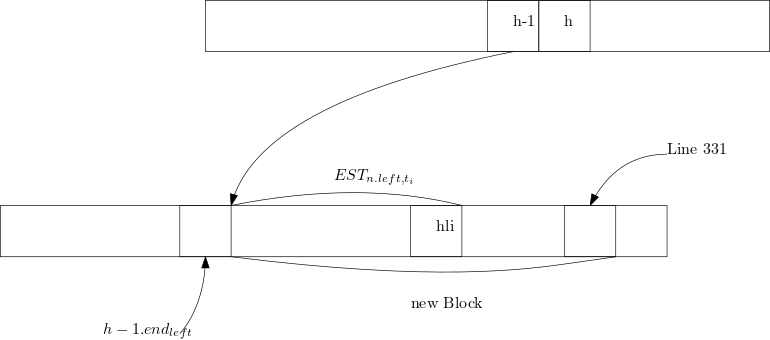
\includegraphics[width=5in]{pics/trueRefresh}
%   \caption{TODO :: Is this picture good or should I remove it? New established operations of the left child are in the new block.(TO UPDATE)}
% \end{figure}

\begin{corollary}\label{lem::prectrueRefresh}
If $R$ is a complete instance \nf{$n$.Refresh}, then we have $EST_{n\nf{.left}}^{t^R} \; \cup \; EST_{n\nf{.right}}^{t^R} \subseteq EST_{n}^{^Rt}$.
\end{corollary}
\begin{proof}
The left hand side is the same as Lemma \ref{lem::trueRefresh}, so it is sufficient to show when $R$ terminates the established blocks in $n$ are a superset of $n$\nf{.blocks}$_{\ref{cas}}$. Line \ref{cas} writes the block \nf{new} in $n$\nf{.blocks[$h$]} where $h$ is value of $n$\nf{.head} read at Line \ref{readHead}.  Because of Lemma \ref{lem::headInc}  we are sure that $n\nf{.head}>h$ when $R$ terminates. So the block \nf{new} appended to $n$ at Line \ref{cas} is established at $^Rt$. 
\end{proof}

\pagebreak

In the next lemma we show that if two consecutive instances of \nf{Refresh} by the same process on node $n$ fail, then the blocks established in the children of $n$ before the first \nf{Refresh} are guaranteed to be in $n$ after the second \nf{Refresh}.

\begin{lemma} \label{doubleRefresh}
  Consider two consecutive terminating instances $R_1$, $R_2$ of \nf{Refresh} on internal node $n$ by process $p$. If neither $R_1$ nor $R_2$ is a successful \nf{Refresh}, then we have $EST_{n\nf{.left}}^{t^{R{_1}}} \; \cup \; EST_{n\nf{.right}}^{t^{R{_1}}} \subseteq EST_{n}^{^{R{_2}}t}$.
\end{lemma}
\begin{proof}
Let $R_1$ read $i$ from $n\nf{.head}$ at Line \ref{readHead}. By Lemma \ref{lem::headInc}, $R_1$ and $R_2$ both cannot read the same value $i$. By Observation \ref{nonDecreasingHead}, $R_2$ reads a larger value of $n$\nf{.head} than $R_1$.

Consider the case where $R_1$ reads $i$ and $R_2$ reads $i+1$ from Line \ref{readHead}. As $R_2$'s \nf{CAS} in Line \ref{cas} returns \nf{false}, there is another successful instance $R_2^\prime$ of \nf{$n$.Refresh} that has done a \nf{CAS} successfully into \nf{$n$.blocks[$i+1$]} before $R_2$ tries to \nf{CAS}. $R_2^\prime$ creates its block \nf{new} after reading the value $i+1$ from $n$\nf{.head} (Line \ref{readHead}) and $R_1$ reads the value $i$ from $n$\nf{.head}. By Observation \ref{nonDecreasingHead} we have $^{R_1}t<t^{R_1}_{\ref{readHead}}< t^{R2^\prime}_{\ref{readHead}}$ (see Figure \ref{fig::doubleRefresh}). By Lemma \ref{lem::prectrueRefresh} we have 
$EST^{n.\nf{left}}_{^{R_2^\prime}_{\ref{readHead}}t} \cup EST^{n.\nf{right}}_{^{R_2^\prime}_{\ref{readHead}}t} \subseteq ops(n.\nf{blocks}_{t_{\ref{cas}}^{R_2^\prime}})$. Also by Lemma \ref{lem::headInc} on $R_2$, the value  of \nf{n.head} is more than $i+1$ after $R_2$ terminates, so the block appended by $R_2^\prime$ to \nf{n} is established by the time $R_2$ terminates. To summarize, $^{R_1}t$ is before $R_2^\prime$'s read of \nf{$n$.head} ($t_{\ref{readHead}}^{R_2^\prime}$) and $R_2^\prime$'s successful \nf{CAS} ($t^{R_2^\prime}_{\ref{cas}}$) is before $R_2$'s termination ($t^{R_2}$), so by Observation and Lemma \ref{lem::headInc} we have \ref{lem::blocksOrder} $EST_{n.\nf{left}}^{t^{R_1}} \cup EST_{n.\nf{right}}^{t^{R_1}} \subseteq ops(n.\nf{blocks}_{t^{R_2^\prime}_{\ref{cas}}}) \subseteq EST_{n.\nf{left}}^{^{R_2}t}$. 

   If $R_2$ reads some value greater than $i+1$ in Line \ref{readHead} it means $n\nf{.head}$ has been incremented  more than two times since $_{\ref{readHead}}^{R_1}t$. By Lemma \ref{lem::headPosition}, when $n.$\nf{head} is incremented from $i+1$ to $i+2$, $n\nf{.blocks[i+1]}$ is non-null. Let $R_3$ be the \nf{Refresh} on $n$ that has put the block in $n\nf{.blocks[}i+1\nf{]}$. $R_3$ read $n\nf{.head}=i+1$ at Line \ref{readHead} and has put its block in $n\nf{.blocks[}i+1\nf{]}$ before $R_2$'s read of $n.$\nf{head} at Line \ref{readHead}. So we have $t^{R_1}<_{\ref{readHead}}^{R_3}t<_{\ref{cas}}^{R_3}t<t^{R_2}_{\ref{readHead}}<^R_{2}t$. From Observation \ref{lem::blocksOrder}  on the operations before and after $R_3$'s \nf{CAS} and Lemmas \ref{lem::trueRefresh}, \ref{lem::headInc} on $R_3$ the claim holds.
\end{proof}

\begin{figure}[hbt]
  \center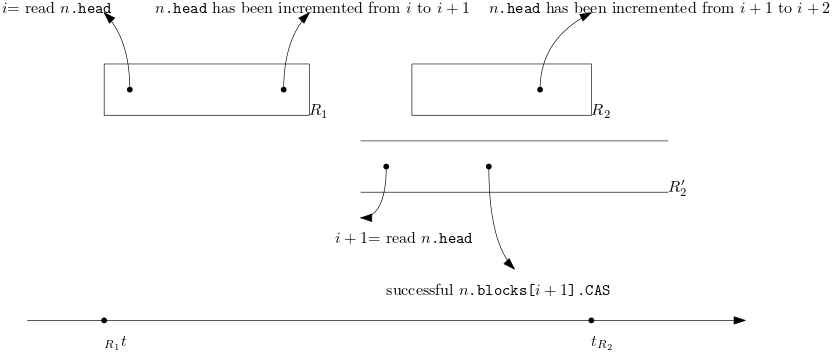
\includegraphics[width=6in]{pics/compactdouble.png}
  \caption{\label{fig::doubleRefresh}$_{R_1}t<$ $t_{\ref{readHead}}^{R_1}$ $<$ incrementing \nf{$n$.head} from $i$ to $i+1$ $<$ $t_{\ref{readHead}}^{R_2^\prime}$ $<$ $t_{\ref{cas}}^{R_2^\prime}$ $<$ incrementing \nf{$n$.head} from $i+1$ to $i+2$ $<t_{R_2}$} 
\end{figure}

\begin{corollary} \label{lem::propagateStep}
  $EST_{n\nf{.left}}^{_{\ref{firstRefresh}}t} \cup EST_{n\nf{.right}}^ {_{\ref{firstRefresh}}t} \subseteq EST_{n}^{t_{\ref{secondRefresh}}}$
\end{corollary}
\begin{proof}
  If the first \nf{Refresh} in line \ref{firstRefresh} returns \nf{true} then by Lemma \ref{lem::prectrueRefresh} the claim holds. If the first \nf{Refresh} failed and the second \nf{Refresh} succeeded the claim still holds by Lemma \ref{lem::prectrueRefresh}. Otherwise both failed and the claim is satisfied by Lemma \ref{doubleRefresh}.
\end{proof}

Now we show that after \nf{Append($b$)} on a leaf finishes, the operation contained in $b$ will be established in \nf{root}.

\begin{corollary}\label{lem::append}
For $A=l\nf{.Append(}b\nf{)}$ we have ${ops(b)} \subseteq EST_{n}^{t^A}$ for each node $n$ in the path from $l$ to \nf{root}.
\end{corollary}
\begin{proof}
$A$ adds $b$ to the assigned leaf of the process, establishes it at Line \ref{appendEnd} and then calls \nf{Propagate} on the parent of the leaf where it appended $b$. For every node $n$, $n.$\nf{Propagate} appends $b$ to $n$, establishes it in $n$ by Corollary \ref{lem::propagateStep} and then calls $n.$\nf{parent.Propagate} untill $n$ is \nf{root}.
\end{proof}

\begin{corollary}\label{lem::appendExactlyOnce}
 After $l$\nf{.Append($b$)} finishes, $b$ is subblock of exactly one block in each node along the path from $l$ to the \nf{root}.
\end{corollary}
\begin{proof}
By the previous corollary and Lemma \ref{lem::appendExactlyOnce} there is exactly one block in each node containing $b$.
\end{proof}

\pagebreak

\subsection{Correctness of GetEnqueue}

First we prove some claims about the size and operations of a block. These lemmas will be used later for the correctness and analysis of \nf{GetEnqueue()}.

\begin{lemma}\label{blockSize}
Each block contains at most one operation of each process, and therefore at most $p$ operations in total.
\end{lemma}
\begin{proof}
To derive a contradiction, assume there are two operations $op_1$ and $op_2$ of process $p$ in block $b$ in node $n$. Without loss of generality $op_1$ is invoked earlier than $op_2$. Process $p$ cannot invoke more than one operation concurrently, so $op_1$ has to be finished before $op_2$ begins. By Corollary \ref{lem::appendExactlyOnce}, before $op_2$ calls \nf{Append}, $op_1$ exists in every node of the tree on the path from $p$'s leaf to the root. Since $b$ contains $op_2$, it must be created after $op_2$ is invoked. This means there is some block $b^\prime$ before $b$ in $n$ containing $op_1$. The existence of $op_1$ in $b$ and $b^\prime$ contradicts Lemma \ref{lem::noDuplicates}.
\end{proof}

\begin{lemma}\label{subBlocksBound}
Each block has at most $p$ direct subblocks.
\end{lemma}
\begin{proof}
The claim follows directly from Lemma \ref{blockSize} and the observation that each block appended to an internal node contains at least one operation, due to the test on Line~\ref{addOP}. We can also see the blocks in the leaves have exactly one operation in the \nf{Enqueue} and \nf{Dequeue} routines.
\end{proof}

\nf{DSearch($e$, $end$)} returns a pair \nf{<$b$, $i$>} such that the $i$th \nf{Enqueue} in the $b$th block of the root is the $e$th \nf{Enqueue} in the entire sequence stored in the root. 
\begin{lemma}[\nf{DSearch} Correctness]\label{dsearch}
If $\nf{root.blocks[$end$]}\neq \nf{null}$ and $1\leq e \leq \nf{root.blocks[$end$].sum\sub{enq}}$, \nf{DSearch($e$, $end$)} returns \nf{<$b$, $i$>} such that $E_i(root,b)= E_e(root)$.
\end{lemma}
\begin{proof}
 From Lines \ref{setSumEnqLeft} and \ref{setSumEnqRight} we know the \nf{sum\sub{enq-left}} and \nf{sum\sub{enq-right}} fields of \nf{blocks} in each node are sorted in non-decreasing order. Since $\nf{sum\sub{enq}}=\nf{sum\sub{enq-left}}+ \nf{sum\sub{enq-right}}$, the $\nf{sum\sub{enq}}$ values of \nf{root.blocks[$0\cdot\cdot end$]} are also non-decreasing. Furthermore, since $\nf{root.blocks[$0$].sum\sub{enq}}=0$ and $\nf{root.blocks[$end$].sum\sub{enq}} \geq e$, there is a $b$ such that $\nf{root.blocks[$b$].sum\sub{enq}} \geq e$ and $\nf{root.blocks[$b-1$].sum\sub{enq}} < e$ by Lemma \ref{lem::sumX}. Block \nf{root.blocks[$b$]} contains $E_i(root,b)$.  Lines \ref{dsearchStart}--\ref{dsearchEnd} doubles the search range in Line \ref{doubling} and will eventually reach \nf{start} such that $\nf{root.blocks[start].sum\sub{enq}}\leq e \leq\nf{root.blocks[end].sum\sub{enq}}$. Then, in Line \ref{dsearchBinarySearch}, the binary search finds the $b$ such that \nf{root.blocks[$b-1$].sum\sub{enq}$<e\leq$root.blocks[$b$].sum\sub{enq}}. By Corollary \ref{lem::sumX}, \nf{root.blocks[$b$]} is the block that contains $E_e(root)$. Finally $i$ is computed using the definition of \nf{sum\sub{enq}} and Corollary \ref{lem::sumX}.
\end{proof}


\begin{lemma}[\nf{GetEnqueue} correctness] \label{get}
If $1\leq i \leq \nf{$n$.blocks[$b$].num\sub{enq}}$ then \nf{$n$.GetEnqueue($b$, $i$)} returns $E_i(n,b)$\nf{.element}.
\end{lemma}
\begin{proof}
We are going to prove this lemma by induction on the height of node $n$. For the base case, suppose $n$ is a leaf. Leaf blocks each contain exactly one operation, $n\nf{.blocks[$b$].sum\sub{enq}}\leq 1$, which means only \nf{$n$.GetEnqueue(b,1)} can be called when $n$ is a leaf. Line \ref{getBaseCase} of \nf{$n$.GetEnqueue($b$, $1$)} returns the \nf{element} of the \nf{Enqueue} operation stored in the $b$th block of leaf ${n}$, as required.

For the induction step we prove if \nf{$n$.child.GetEnqueue($b^\prime$, $i$)} returns $E_i(n.\nf{child}, b^\prime)$ then \nf{$n$.GetEnqueue($b$,~$i$)} returns $E_i(n,b)$.  From Definition \ref{ordering} of $E(n,b)$, so operations from the left subblocks come before the operations from the right subblocks in a block (see Figure \ref{figGet}). By Observation \ref{lem::numX}, the \nf{num\sub{enq-left}} field  in \nf{$n$.blocks[$b$]} is the number of \nf{Enqueue} operations from the blocks's subblocks in the left child of $n$. So the $i$th \nf{Enqueue} operation in $n\nf{.blocks[}b\nf{]}$ is propagated from the right child if and only if $i$ is greater than $n\nf{.blocks[}b\nf{]}$\nf{.num\sub{enq-left}}. Line \ref{leftOrRight} decides whether the $i$th enqueue in the $b$th block  of internal node $n$ is in the  left child or right child subblocks of \nf{$n$.blocks[$b$]}. By Definitions \ref{def::subblock} and \ref{def::ops} to find an operation in the subblocks of \nf{$n$.blocks[$i$]} we need to search in the range
\begin{align*}
&\texttt{$n$.left.blocks[$n$.blocks[$i$-1].end\textsubscript{left}+1..$n$.blocks[$i$].end\textsubscript{left}]}  \textrm{ or } \\
&\texttt{$n$.right.blocks[$n$.blocks[$i$-1].end\textsubscript{right}+1..$n$.blocks[$i$].end\textsubscript{right}]}.
 \end{align*}
First we consider the case where the \nf{Enqueue} we are looking for is in the left child. There are $eb=n.\nf{blocks[}b-1\nf{].sum\sub{enq-left}}$ \nf{Enqueue}s in the blocks of $n$\nf{.left} before the left subblocks of $n$\nf{.blocks[$b$]}, so $E_i(n,b)$ is $E_{i+eb}(n.\tt{left})$ which is $E_{i^\prime}(n.\tt{left},b^\prime)$ for some $b^\prime$ and $i^\prime$. We can compute $b^\prime$ and then search for the $i+eb$th enqueue in \tt{n.left}, where $i^\prime$ is $i+eb-n$\tt{.left.blocks[}$b^\prime-1$\tt{].sum\sub{enq}}. The parameters in Line \ref{leftChildGet} are for searching $E_{i+eb}(n.left)$ in \nf{$n$.left.blocks} in the range of left subblocks of $n$\nf{.blocks[}$b$\nf{]}, so this \nf{BinarySearch} returns the index of the subblock containing $E_i(n,b)$.

Otherwise, the enqueue we are looking for is in the right child. Because \nf{Enqueue}s from the left subblocks are ordered before the \nf{Enqueue}s from the right subblocks, there are \nf{n.blocks[b].num\sub{enq-left}} enqueues ahead of $E_i(n,b)$ from the left child. So we need to search for $i-n\nf{.blocks[}b\nf{].num\sub{enq-left}}+ n\nf{.blocks[}b-1\nf{].sum\sub{enq-right}}$ in the right child (Line \ref{rightChildGet}). Other parameters for the right child are chosen similarly to the left child. 

So, in both cases the direct subblock containing $E_i(n,b)$ is computed in Line \ref{leftChildGet} or \ref{rightChildGet}.
 Finally, \nf{$n$.child.GetEnqueue($subblock$, $i$)} is invoked on the subblock containing $E_i(n,b)$ and it returns $E_i(n,b)$\nf{.element} by the hypothesis of the induction.
\end{proof}

\begin{figure}[hbt]  
  \center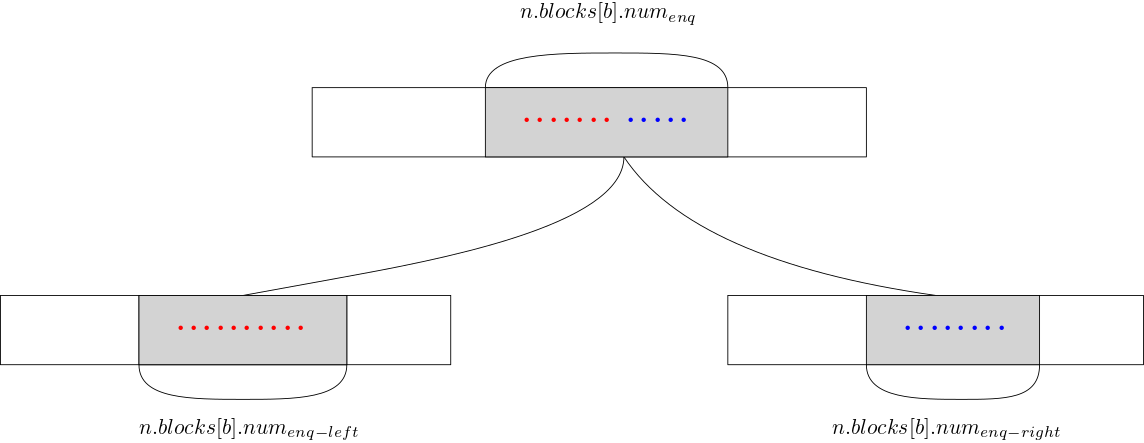
\includegraphics[width=6in]{pics/blockSumEnq.png}
  
  \caption{The number and ordering of the enqueue operations propagated from the left and the right child to \nf{$n$.blocks[$b$]}. Both \nf{$n$.blocks[$b$]} and its subblocks are shown in grey. \nf{Enqueue} operations from the left subblocks (colored red), are ordered before the \nf{Enqueue} operations from the right child (colored blue).
  }\label{figGet}
\end{figure}

\clearpage

\subsection{Correctness of IndexDequeue}
The next few results show that the \nf{super} field of a block is accurate within one of the actual index of the block's superblock in the parent node. Then we explain how it is used to compute the rank of a given \nf{Dequeue} in the root.
\begin{definition}\label{orderRefresh} If a \nf{Refresh} instance $R_1$ does its \nf{CAS} at Line \ref{cas} earlier than \nf{Refresh} instance $R_2$ we say $R_1$ has \it{happened before} $R_2$.
\end{definition}

\begin{observation} \label{setSupBeforeIncHead}
After \nf{$n$.blocks[$i$].CAS(null, $B$)} succeeds, \nf{$n$.head} cannot increase from ${i}$ to ${i+1}$ until \nf{$B$.super} is set.
\end{observation}
\begin{proof}
From Observation \ref{nonDecreasingHead} we know the \nf{$n$.head} changes only by the increment on Line \ref{incrementHead}. Before an instance of \nf{Advance} increments \nf{n.head} on Line \ref{incrementHead}, Line \ref{setSuper1} ensures that \nf{n.blocks[head].super} was set at Line \ref{setSuper1}.
\end{proof}

\begin{corollary}
  If \nf{$n$.blocks[$i$].super} is \nf{null}, then $\nf{$n$.head}\leq i$ and \nf{$n$.blocks[$i+1$]} is \nf{null}.
\end{corollary}
\begin{proof}
By Lemma \ref{lem::headPosition} and Observation \ref{setSupBeforeIncHead}.
\end{proof}
Now let us consider how the \nf{Refresh}es that took place on the parent of node $n$ after block $B$ was stored in $n$ will help to set \nf{$B$.super} and propagate $B$ to the parent.

\begin{observation}\label{lem::createBlockHead}
If the block created by an instance $R_p$ of $n$\nf{.parent.Refresh} contains block $B=n$\nf{.blocks[}$b$\nf{]} then $R_p$ reads a value greater than $b$ from $n$\nf{.head} in Line \ref{lastLine}. 
\end{observation}

\begin{lemma}
  If $B=n$\nf{.blocks[}$b$\nf{]} is a direct subblock of \nf{$n$.parent.blocks[$sb$]} then $\nf{$B$.super}\leq sb$.
\end{lemma}
\begin{proof}
Let $R_p$ be the instance of $n$\nf{.parent.Refresh} that stores $n$\nf{.parent.blocks[$sb$]}. By \ref{lem::createBlockHead} if $R_p$ propagates $B$ it has to read a greater value than $b$ from \nf{$n$.head}, which means \nf{$n$.head} was incremented from $b$ to $b+1$ in Line \ref{incrementHead}. By Observation \ref{setSupBeforeIncHead} \nf{$B$.super} was already set in Line \ref{setSuper1}. The value written in \nf{$B$.super} was read in Line \ref{readParentHead},s before the \nf{CAS} that sets \nf{$B$.super}. From Observation \ref{nonDecreasingHead} we know \nf{$n$.parent.head} is non-decreasing so $B\nf{.super}\leq sb$, since \nf{$n$.parent.head} is still equal to $sb$ when $R_p$ executes its \nf{CAS} at Line \ref{cas} by Invariant \ref{lem::headProgress}. The reader may wonder when the case $b\nf{.super}=sb$ happens. This can happen when $\nf{$n$.parent.blocks[$B$.super]}=\nf{null}$ when $B$\nf{.super} is written and $R_p$ puts its created block into \nf{$n$.parent.blocks[$B$\nf{.super}]} afterwards.
\end{proof}

\begin{lemma}
Let $R_n$ be a \nf{Refresh} that puts $B$ in \nf{$n$.blocks[$b$]} at Line \ref{cas}. Then, the block created by one of the next two successful \nf{$n$.parent.Refresh}es according to Definition \ref{orderRefresh} contains $B$ and \nf{$B$.super} is set when the second successful \nf{$n$.parent.Refresh} reaches Line \ref{invokeCreateBlock}.
\end{lemma}

\begin{proof}
Let $R_{p1}$ be the first successful \nf{$n$.parent.Refresh} after $R_n$ and $R_{p2}$ be the second next successful \nf{$n$.parent.Refresh}. To derive a contradiction assume $B$ was not propagated to $n$\nf{.parent} by $R_{p1}$ nor by $R_{p2}$.

Since $R_{p2}$'s created block does not contain $B$, by Observation \ref{lem::createBlockHead} the value $R_{p2}$ reads from $n$\nf{.head} in Line \ref{lastLine} is at most $b$. From Observation \ref{nonDecreasingHead} the value $R_{p2}$ reads in Line \ref{readChildHead} is also at most $b$.

$R_n$ puts $B$ into $n$\nf{.blocks[}$b$\nf{]} so ${R_n}$ reads the value $b$ from $n.$\nf{head}. Since $R_{p2}$'s \nf{CAS} into $n$\nf{.parent.blocks} is successful there should be a \nf{Refresh} instance $R_p^\prime$ on $n$\nf{.parent} that increments $n$\nf{.parent} (Line \ref{incrementHead}) after $R_{p1}$'s Line \ref{cas} and before $R_{p2}$'s Line \ref{readHead}. We assumed $t^{R_n}_{\ref{cas}}<t^{R_{p1}}_{\ref{cas}}<t^{R_{p2}}_{\ref{cas}}$ by Definition \ref{orderRefresh}. Finally, Line \ref{readChildHead} is after Line \ref{readHead} and $R_{p2}$'s \ref{readHead} is after $R_p^\prime$'s Line \ref{incrementHead}, which is after ${R_n}$'s $n$\nf{.blocks.CAS}. 
\begin{align*}
\left.
\begin{array}{r}
 _{\ref{cas}}^{R_n}t<_{\ref{cas}}^{R_{p1}}t\\
_{\ref{cas}}^{R_{p1}}t<_{\ref{incrementHead}}^{R_{p^\prime}}t<_{\ref{readHead}}^{R_{p2}}t\\
_{\ref{readHead}}^{R_{p2}}t<_{\ref{readChildHead}}^{R_{p2}}t\\
\end{array}
\right\} &\Longrightarrow  _{\ref{cas}}^{R_n}t<_{\ref{readChildHead}}^{R_{p2}}t
\end{align*}

So $R_{p2}$ reads a value greater than or equal to $b$ for $n.\nf{head}$ by Lemma \ref{nonDecreasingHead}.

Therefore $R_{p2}$ reads $n\nf{.head}=b$. $R_{p2}$ calls $n$\nf{.Advance} at Line Line \ref{helpAdvance}, which ensures $n$\nf{.head} is incremented from $b$. So the value $R_{p2}$ reads in Line \ref{lastLine} of \nf{CreateBlock} is greater than $b$ and $R_{p2}$'s created block contains $B$. This is contradiction with our hypothesis.

Furthermore, if $B$\nf{.super} was not set earlier it is set by $R_{p2}$ call to $n$\nf{.Advance} invoked from Line \ref{helpAdvance}.

% \nf{$b$.super} is set by some instance of \nf{Refresh} on $n$ or \nf{$n$.parent} showed by $R^\prime$ and \nf{$n$.head} is incremented by some \nf{Refresh} called $R^\prime\prime$. Let \nf{$n$.parent.head} value be $hp$ when $R^\prime$ reads it. From Lemma \ref{lem::headProgress} \nf{$n$.parent.head} could only increase from ${hp}$ to ${hp+1}$ if $\nf{$n$.parent.blocks[$hp$]}\neq\nf{null}$. In other words there should be a successful \nf{$n$.parent.Refresh} for \nf{$n$.parent.head} to be increased. Let $R_p$ be \nf{$n$.parent.Refresh} that propagated $b$ to \nf{$n$.parent}. We claim there cannot be another successful \nf{$n$.parent.Refresh} after $R^\prime$ reads \nf{$n$.parent.head} and before $R_p$ performs Line \ref{lastLine}.

% \begin{figure}[hbt]  
%   \center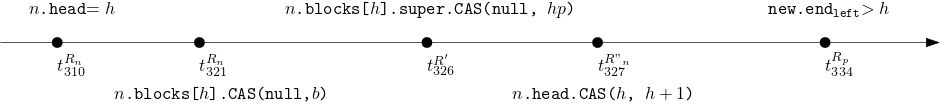
\includegraphics[width=5.5in,height=0.65in]{pics/timeLineSuper1.png}
%   \caption{Time relations between \nf{R\sub{n},R\sub{p},R',R"}}
%   \label{fig::timeLine1}
% \end{figure}

% Without loss of generality  assume $n$ is the left child of \nf{$n$.parent}. As we mentioned the first successful \nf{$n$.parent.Refresh} after $t_{\ref{cas}}^{Rn}$ did not set \nf{$b$.super}. It might happen maybe because the value $h_{left}$ read for $n$\nf{.head} in Line \ref{readChildHead} is less than or equal to $i$ and $\nf{left.blocks[$h_{left}$]}=\nf{null}$, which means \nf{$n$.head} is advanced but $b$ is still not installed in \nf{$n$.blocks[$i$]} which means $R_n$ has not reached  the Line \ref{cas}.
  
% Let the first successful \nf{$n$.parent.Refresh} be $R_{p1}$ and the second next successful \nf{$n$.parent.Refresh} be $R_{p2}$. If $R_{p1}$ reads $x$ in Line \ref{readHead}, then $R_{p2}$ has to read ${x+1}$ in Line \ref{readHead} (induced from \ref{lem::headProgress}, \ref{nonDecreasingHead}). See the timeline in Figure \ref{fig::timeLine2} for two consecutive successful \nf{Refresh} instances $R_{p1}$,$R_{p2}$ on \nf{$n$.parent}.

% \begin{figure}[hbt]  
%   \center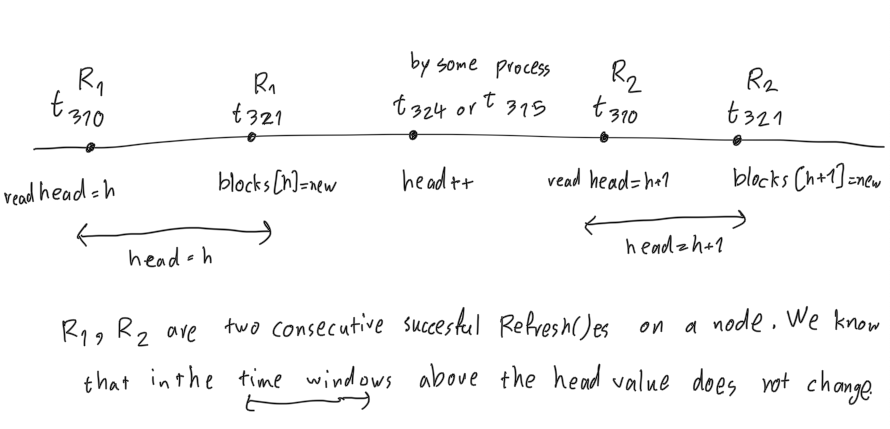
\includegraphics[width=6in,height=1.25in]{pics/timeLineSuper2.png}
%   \caption{$R_{p2}$ reads \nf{$n$.parent.head} after $t_{320}^{R_{p1}}$, which is after $t_{320}^{Rn}$. $R_{p2}$ has to help increment \nf{$n$.head} and set $b$\nf{.super}.}
%   \label{fig::timeLine2}
% \end{figure}


% $$t_{\ref{cas}}^{R_n}<t_{\ref{cas}}^{R_p}<t_{\ref{cas}}^{R_p'}<t_{314}^{R_p'}$$
% $t_{\ref{cas}}^{R_n}<t_{\ref{cas}}$ because $R_p$ is the first successful $p.Refresh$ after $R_n$. $t_{\ref{cas}}^{R_p}<t_{\ref{cas}}^{R_p'}$ because of the time windows between two consecutive successful \nf{Refresh} instances on a node. $t_{\ref{cas}}^{R_p'}<t_{314}^{R_p'}$ because it is sequential in the code. The second Refresh on \nf{p} contains $b$ and reads $\nf{n.head}>\nf{i}$.

% So \nf{$b$.super} has set by some process before the second next successful \nf{$n$.parent.Refresh} on Line \ref{setSuper1}. Since $i$ is read in the Line \ref{readHead} then the \nf{CreateBlock} in Line \ref{invokeCreateBlock} is going to read  some value for \nf{left.head} greater than ${h}$ and propagates $b$ to \nf{$n$.parent}. So if $b$ was not propagated already we are sure the second next successful \nf{$n$.parent.Refresh} propagates $b$.
\end{proof}

\begin{corollary} \label{superRelation}
If \nf{$B=n$.blocks[$b$]} is propagated to $n$\nf{.parent}, then \nf{$B$.super} is equal to or one less than the index of the superblock of $B$.
\end{corollary}
\begin{proof}
% After that $B$ is installed $n$\nf{.parent.head} is read and $B.$\nf{super} field is set to the value read from the parent's \nf{head} (see Lines \ref{readParentHead} and \ref{setSuper1} of\nf{Advance}).
Let $R_n$ be the \nf{$n$.Refresh} that put $B$ in $n$\nf{.blocks} and let $R_{p1}$ be the first successful \nf{$n$.parent.Refresh} after $R_n$ and $R_{p2}$ be the second next successful \nf{$n$.parent.Refresh}.
Before  $B$ can be propagated to $n$'s \nf{parent}, $n$\nf{.head}  must be greater than $b$, so by Observation \ref{setSupBeforeIncHead} $B$\nf{.super} is set.
From thr previous Lemma we know that $B$ is propagated by second next successful \nf{Refresh}'s \nf{CAS} on $n$\nf{.parent.blocks}. To summarize we have $n\nf{.parent.head}_{_{\ref{cas}}^{R_{p2}}t}= n\nf{.parent.head}_{_{\ref{cas}}^{R_{p1}}t}+1$ and by Definition \ref{orderRefresh} and Observation \ref{nonDecreasingHead} $n\nf{.parent.head}_{_{\ref{cas}}^{R_{p1}}t}\leq n\nf{.parent.head}_{_{\ref{cas}}^{R_n}t}$. The value that is set in $B$\nf{.super} is read from $n$\nf{.parent.head} after ${_{\ref{cas}}^{R_n}t}$. So $B$\nf{.super} is equal to or one less than the index of the superblock of $B$.
\end{proof}

Now using Corollary \ref{superRelation} on each step of the \nf{IndexDequeue} we prove its correctness.

\begin{lemma}[\nf{IndexDequeue} correctness]
 If $1\leq i \leq\nf{$n$.blocks[$b$].num\sub{deq}}$ then \nf{$n$.IndexDequeue($b$,$i$)} returns $<x,y>$ such that $D_i(n,b)=D_y(\nf{root},x)$.
\end{lemma}
\begin{proof}
We will prove this by induction on the distance of $n$ from the \nf{root}. The base case where $n$ is \nf{root} is trivial (see Line \ref{indexBaseCase}).
For the non-root nodes \nf{$n$.IndexDequeue($b$, $i$)} computes $sb$, the index of the superblock of the $b$th block in $n$, in Line \ref{computeSuper} by Corollary \ref{superRelation}. After that, the position of $D_i(n,b)$ in $D(n.\nf{parent}, sb)$ is computed in Lines \ref{computeISuperStart}--\ref{computeISuperEnd}. By Definition \ref{ordering}, \nf{Dequeue}s in a block are ordered based on the order of its subblocks  from left to right. If $D_i(n,b)$ was propagated from the left child, the number of dequeus in the left subblocks of \nf{$n$.parent.blocks[$sb$]} before \nf{$n$.blocks[$b$]} is considered in Line \ref{considerPreviousLeft} (see Figure \ref{fig::blockSumDeqLeft}). Otherwise, if $D_i(n,b)$ was propagated from the right child, the number of dequeues in the subblocks from the left child is considered to be ahead of the computed index (Line \ref{considerRight}) (see Figure \ref{fig::blockSumDeqRight}). Finally \nf{IndexDequeue} is called on \nf{$n$.parent} recursively and it returns the correct response by induction hypothesis. 
\end{proof}
\begin{figure}[hbt]  
  \center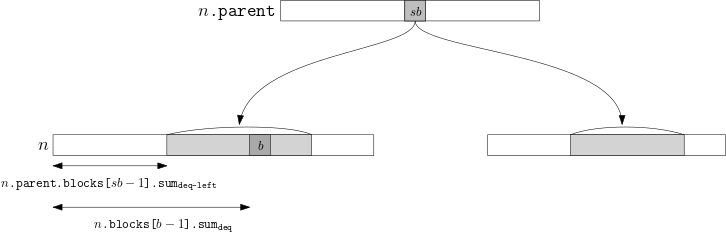
\includegraphics[width=6in]{pics/blockSumDeqLeft.png}
  
  \caption{The number of \nf{Dequeue} operations before $E_i(n,b)$ shown in the case where $n$ is a left child.}\label{fig::blockSumDeqLeft}
\end{figure}
\begin{figure}[hbt]  
  \center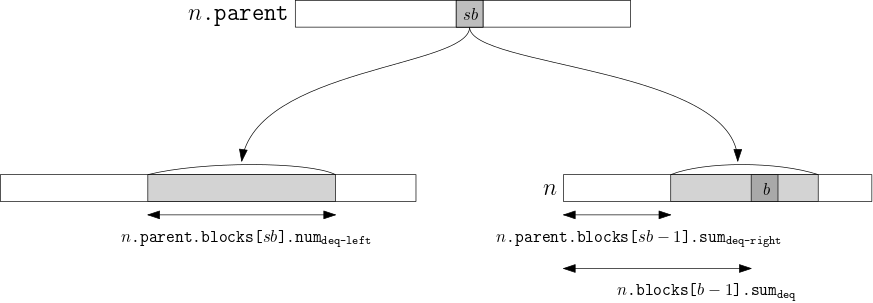
\includegraphics[width=6in]{pics/blockSumDeqRight.png}
  
  \caption{The number of \nf{Dequeue} operations before $E_i(n,b)$ shown in the case where $n$ is a right child.}\label{fig::blockSumDeqRight}
\end{figure}

\pagebreak
\subsection{Linearizability}
We now prove the two properties needed for linearizability.

\begin{lemma} \label{linearSat}
$L$ is a legal linearization ordering.
\end{lemma}
\begin{proof}
We must show that, every operation that terminates is in $L$ exactly once and if $op_{1}$ terminates before $op_{2}$ starts in execution then $op_{1}$ is before $op_{2}$ in the linearization. The first claim is directly reasoned from Lemma \ref{lem::appendExactlyOnce}. For the latter, if $op_{1}$ terminates before $op_{2}$ starts,  $op_{1}$\nf{.Append} has terminated before $op_{2}$\nf{.Append} started. From Lemma \ref{lem::append}, $op_{1}$ is in \nf{root.blocks} before $op_{2}$ starts to propagate. By definition of $L$, $op_{1}$ is linearized before $op_{2}$.
\end{proof}
Once some operations are aggregated in one block, they will get propagated up to the root together and they can be linearized in any order among themselves. We have chosen to put \nf{Enqueue}s in a block before \nf{Eequeue}s (see Definition \ref{ordering}).

\begin{definition}\label{defNullDeq}
If a \nf{Dequeue} operation returns\nf{null} it is called a \it{null} \nf{Dequeue}, otherwise it is called \it{non-null} \nf{Dequeue}.
\end{definition}

Next we define  the responses that \nf{Dequeue}s should return, according to the linearization.
\begin{definition}
   Assume the operations in \nf{root.blocks} are applied sequentially on an empty queue in the order of $L$.  ${Resp(d)=e}$\nf{.element} if the element of \nf{Enqueue} $e$ is the response to \nf{Dequeue} $d$. Otherwise if ${d}$ is a\nf{null} dequeue then ${Resp(d)=\nf{null}}$. 
\end{definition}

% \begin{observation}\label{enqBeforeDeq}
% By Definition \ref{ordering} \nf{Enqueue} operations come before \nf{Dequeue} operations in a block.  
% \end{observation}

In the next lemma we show that the \nf{size} field in each \nf{root block} is computed correctly.
\begin{lemma}\label{sizeCorrectness}
  \nf{root.blocks[$b$].\size}is the \size of the queue if the operations in \nf{root.blocks[$0\cdots b$]} are applied in the order of~$L$.  
\end{lemma}
\begin{proof}
We prove the claim by induction on $b$. The base case when ${b=0}$ is trivial since the queue is initially empty and $\nf{root.blocks[}0\nf{].size}=0$. We are going to show the correctness when $b=i$ assuming  correctness when $b=i-1$. By Definition \ref{ordering} \nf{Enqueue} operations come before \nf{Dequeue} operations in a block. By Lemma \ref{lem::numX} \nf{num\sub{enq}} and \nf{num\sub{deq}} fields in a block show ther number of \nf{Enqueue} and \nf{Dequeue} operations in it. If there are more than $\nf{root.blocks[}i-1\nf{].size}+\nf{root.blocks[}i\nf{].num\sub{enq}}$ dequeue operations in \nf{root.blocks[$i$]} then the queue would become empty after \nf{root.blocks[$i$]}. Otherwise the size of the queue after the $b$th block in the root is $\nf{root.blocks[}b-1\nf{].size}+ \nf{root.blocks[}b\nf{].num\sub{enq}}- \nf{root.blocks[}b\nf{].num\sub{deq}}$. In both cases, this is same as the assignment on Line \ref{computeLength}.
\end{proof}

The next lemma is useful to compute the number of non-null dequeues.
\begin{lemma} \label{numberOfNND}
If operations in the root are applied with the order of $L$, the number of non-null \nf{Dequeue}s in $\nf{root.blocks[}0\cdots b\nf{]}$ is \nf{root.blocks[$b$].sum\sub{enq} $-$ root.blocks[$b$].size}.
\end{lemma}
\begin{proof}
There are \nf{root.blocks[$b$]}\nf{.sum\sub{enq}} enqueue operations in $\nf{root.blocks[}0\cdots b\nf{]}$. The size of the queue after doing $\nf{root.blocks[}0\cdots b\nf{]}$ in order $L$ is 
the number of $\it{enqueues}$ in $\nf{root.blocks[}0\cdots b\nf{]}$ minus the number of $\it{non-null \nf{Dequeue}s}$ in $\nf{root.blocks[}0\cdots b\nf{]}$. By the correctness of the \nf{size} field from Lemma \ref{sizeCorrectness} and \nf{sum\sub{enq}} field from Lemma \ref{lem::numX}, the number of $\it{non-null \nf{Dequeue}s}$ is \nf{root.blocks[$b$]}\nf{.sum\sub{enq}} $-$ \nf{root.blocks[$b$]}\nf{.size}. 
\end{proof}

\begin{corollary}\label{numNullDeqBlock}
  If operations in the root are applied with the order of $L$, the number of non-null dequeues in $\nf{root.blocks[}b\nf{]}$ is \nf{root.blocks[$b$].num\sub{enq} $-$ root.blocks[$b$].\size $+$ root.blocks[$b-1$].size}.
\end{corollary}

\begin{lemma}\label{nullReturn}
$Resp(D_i(\nf{root},b))$ is \nf{null} iff \nf{root.blocks[$b-1$].\size $+$ root.blocks[$b$].num\sub{enq}$- i$ $<0$}.
\end{lemma}
\begin{proof}
From Corollary \ref{numNullDeqBlock} and Lemma \ref{lem::numX}.
\end{proof}

\begin{lemma}\label{computeHead}
\nf{FindResponse($b$, $i$)} returns $Resp(D_i(root,b))$.
\end{lemma}
\begin{proof}
$D_i(root,b)$ is $D_{\nf{root.blocks[}b-1\nf{].sum\sub{deq}}+i}(root)$ by Definition \ref{ordering} and Lemma \ref{lem::sumX}. $D_i(root,b)$ returns \nf{null} at Line \ref{returnNull} if $\nf{root.blocks[}b-1\nf{].size}+ \nf{root.blocks[}b\nf{].num\sub{enq}}- i <0$ and $Resp(D_i(root,b))=\nf{null}$ in this case by Lemma \ref{nullReturn}. Otherwise, if $D_i(root,b)$ is the $e$th non-null dequeue in $L$ it should return the $e$th enqueued value. By Lemma \ref{numberOfNND} there are \nf{root.blocks[$b-1$].sum\sub{enq} $-$ root.blocks[$b-1$].\size} non-null \nf{Dequeue} operations in $\nf{root.blocks[}0\cdots b-1\nf{]}$. The \nf{Dequeue}s in \nf{root.blocks[$b$]} before $D_i(root,b)$ are non-null dequeues. So $D_i(root,b)$ is the $e$th non-null \nf{Dequeue} where $e= i + \nf{root.blocks[}b-1\nf{].sum\sub{deq}} - \nf{root.blocks[}b-1\nf{].size}$ (Line \ref{computeE}). See Figure \ref{computeResponseDetail}.

After computing $e$ at Line \ref{computeE}, the code finds \nf{$b$,$i$} such that $E_i(root,b)=E_e(root)$ using \nf{DSearch} and then finds its \nf{element} using \nf{GetEnqueue} (Line \ref{findAnswer}). Correctness of \nf{DSearch} and \nf{GetEnqueue} routines are shown in Lemmas \ref{dsearch} and \ref{get}.
\end{proof}

\begin{figure}[hbt]  
  \center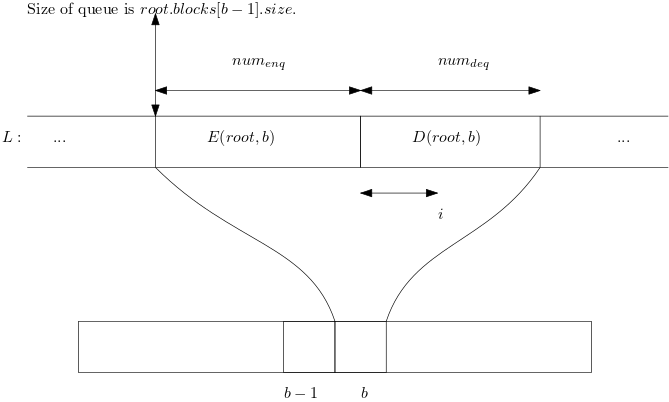
\includegraphics[width=4in, height=2.5in]{pics/computeResponseDetail.png}\caption{The position of $D_i(root,b)$.}
\label{computeResponseDetail}
\end{figure}

\begin{lemma}\label{linearCorrect}
The responses to operations in our algorithm would be the same as in the sequential execution in the order given by $L$.
\end{lemma}
\begin{proof}
\nf{Enqueue} operations do not return any value. By Lemma \ref{computeHead} response of a \nf{Dequeue} in our algorithm is same as the response from the sequential execution of $L$.  
\end{proof}

\begin{theorem}[Main]
The queue implementation is linearizable.
\end{theorem}
\begin{proof}
The theorem follows from Lemmas \ref{linearSat} and \ref{linearCorrect}.
\end{proof}

\paragraph{Remark} In fact our algorithm is strongly linearizable as defined in \cite{DBLP:conf/stoc/GolabHW11}. By Definition \ref{ordering} the linearization ordering of operations will not change as blocks containing new operations are appended to the root.
\pagebreak

\section{Analysis}

Is this a Lemma or a Result or an Observation of Algorithm? Which is not used in main wait-free theorem.
\begin{lemma}
An \nf{Enqueue} or \nf{Dequeue} operation does at most $14\log p$ \nf{CAS} operations.
\end{lemma}
\begin{proof}
  In each level of the tree  \nf{Refresh} is invoked at most two times and  every \nf{Refresh} invokes at most 7 \nf{CAS}es, one in Line \ref{cas} and two from each \nf{Advance} in Line \ref{helpAdvance} or \ref{advance}.
\end{proof}

\begin{lemma}[\nf{DSearch} Analysis]\label{dsearchTime}
If the \nf{element} enqueued by $E_i(root,b)=E_e(root)$ is the response to some \nf{Dequeue} operation in \nf{root.blocks[$end$]}, then \nf{DSearch($e$, $end$)} takes $O\big(\log ( \nf{root.blocks[$b$].size}+ \nf{root.blocks[$end$].size})\big )$ steps.
\end{lemma}
\begin{proof}
First we show $end - b -1\leq 2 \times \nf{root.blocks[$b-1$].size}+\nf{root.blocks[$end$].size}$. There can be at most \nf{root.blocks[$b$].size}  \nf{Dequeue}s in \nf{root.blocks[$b+1\cdots end-1$]}; otherwise all elements enqueued by \nf{root.blocks[$b$]} would be dequeued before \nf{root.blocks[$end$]}. Furthermore in the execution of queue operations in the linearization ordering, the size of the queue becomes \nf{root.blocks[$end$].size} after the operations of \nf{root.blocks[$end$]}. The final size of the queue after \nf{root.blocks[$1\cdots end$]} is \nf{root.blocks[$end$].size}. After an execution on a queue the $size$ of the queue is greater than or equal to $\#enqueues -\#dequeues$ in the execution. We know the number of dequeues in \nf{root.blocks[$b+1\cdots end-1$]} is less than \nf{root.blocks[$b$].size}, therefore in \nf{root.blocks[$b+1\cdots end-1$]} cannot be more than $\nf{root.blocks[$b$].size} + \nf{root.blocks[$end$].size}$ \nf{Enqueue}s. Overall there can be at most $2 \times\nf{root.blocks[$b$].size}+ \nf{root.blocks[$end$].size}$ operations in \nf{root.blocks[$b+1\cdots end-1$]} and since from Line \ref{addOP} we know that \nf{num} field of the every block in the tree is greater than 0, each block has at least one operation, there are at most $2 \times\nf{root.blocks[$b$].size}+ \nf{root.blocks[$end$].size}$ blocks in between \nf{root.blocks[$b$]} and \nf{root.blocks[$end$]}. So $end-b-1\leq 2 \times\nf{root.blocks[$b$].size}+\nf{root.blocks[$end$].size}$.

So, the doubling search reaches \nf{start} such that the \nf{root.blocks[start].sum\sub{enq}} is less than $e$ in $O \big(\log(\nf{root.blocks[$b$].size}+\nf{root.blocks[$end$].size})\big)$ steps. See Figure \ref{fig::doubling}. After Line \ref{dsearchEnd}, the binary search that finds $b$ also takes $O\big(\log(\nf{root.blocks[$b$].size}+\nf{root.blocks[$end$].size})\big)$. Next, \nf{i} is computed via the definition of \nf{sum\sub{enq}} in constant time (Line \ref{DSearchComputei}).
\end{proof}
\begin{figure}[hbt]  
  \center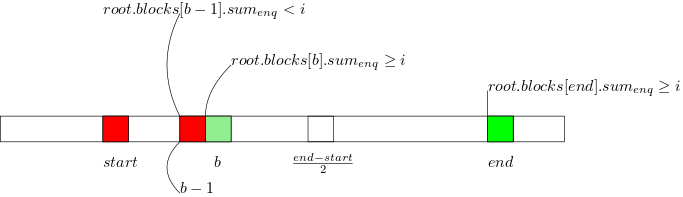
\includegraphics[width=6in]{pics/doubling.png}
  \caption{Distance relations between \nf{start}$,b,end$.}
  \label{fig::doubling}
\end{figure}

\begin{lemma}[Worst Case Time analysis] \label{enqDeqTime}
The worst case number of steps for an \nf{Enqueue} is $O(\log^2 p)$ and for a \nf{Dequeue}, is $O(\log^2 p + \log q_e+ \log q_d)$,  where $q_d$ is the size of the queue when the \nf{Dequeue} is linearized and $q_i$ is the size of the queue at time the response of the \nf{Dequeue} is linearized.
\end{lemma}
\begin{proof}
\nf{Enqueue} consists of creating a block and appending it to the tree. The first part takes constant time. To propagate the operation to the root the algorithm tries at most two \nf{Refresh}es in each node of the path from the leaf to the root (Lines \ref{firstRefresh}, \ref{secondRefresh}). We can see from the code  that each \nf{Refresh} takes a constant number of steps and does $O(1)$ \nf{CAS}es. Since the height of the tree is $\Theta(\log p)$, \nf{Enqueue} takes $O(\log p)$ steps.

A \nf{Dequeue} creates a block whose \nf{element} is \nf{null}, appends it to the tree, computes its rank among non-null dequeues, finds the corresponding enqueue and returns the response. The first two parts are similar to an \nf{Enqueue} operation and take $O(\log p)$ steps. To compute the rank of a \nf{Dequeue} in $D(n)$ the dequeue calls \nf{IndexDequeue()}. \nf{IndexDequeue} does $O(1)$ steps in each level which takes $O(log p)$ steps. If the response to the dequeue is \nf{null}, \nf{FindResponse} returns \nf{null} in $O(1)$ steps. Otherwise, if the response to a dequeue in \nf{root.blocks[end]} is in \nf{root.blocks[b]} the \nf{DSearch} takes $\Theta(\log$(\nf{root.blocks[b].size+root.blocks} \nf{[end].size}) by Lemma \ref{dsearchTime}, which is $O(\log$ size of the queue when \nf{Enqueue} is linearized$)+\log$ size of the queue when \nf{Dequeue} is linearized$)$. Each search in \nf{GetEnqueue()} takes $O(\log p)$ since there are $\leq p$ subblocks in a block (Lemma \ref{subBlocksBound}), so \nf{GetEnqueue()} takes $O(\log^2 p)$ steps.
\end{proof}

\begin{lemma}[Amortized Time Analysis]
The amortized number of steps for an \nf{Enqueue} or \nf{Dequeue}, is $O(\log^2 p + \log q)$,  where $q$ is the size of the queue when the operation is linearized.
\end{lemma}
\begin{proof}
If we split \nf{DSearch} time cost between the corresponding \nf{Enqueue}, \nf{Dequeue}, in each operation takes $O(\log^2 p +q)$ steps.
\end{proof}

\begin{theorem}
The queue implementation is wait-free.
\end{theorem}
\begin{proof}
To prove the claim, it is sufficient to show that every \nf{Enqueue} and \nf{Dequeue} operation terminates after a finite number of its own steps. This is directly concluded from Lemma \ref{enqDeqTime}.
\end{proof}

\pagebreak
\section{Future Directions}
We designed a tree to achieve agreement on an linearization of operations invoked by $p$ processes in an asynchronous model, which we will call \it{Block Tree}. We also implemented two queries to know information about the ordering agreed in the block tree. Then we used the tree to implement a queue where the number of steps per operation is poly-logarithmic with respect to the size of the queue and the number of processes. Block trees can be used as a mechanism to achieve agreement among processes to construct more poly-logarithmic wait-free linearizable objects. In the next paragraphs we talk about possible improvements on block trees and the data structures that we can implement with block trees.

\paragraph{Reducing Space Usage}
The \nf{blocks} arrays defined in our algorithm are unbounded. We could instead use the vector of Feldman, Valera-Leon and  Damian Segment~\cite{7073592} model to use $O(n)$ space in each node, where $n$ is the total number of operations. Their vector creates an array called \nf{arr} of pointers to array segments. When a process wishes to write into \nf{head} it checks whether \nf{arr[$\lfloor\log $ head$\rfloor$]} points to an array or not. If not, it creates a shared array with size $2^{\lfloor\log \nf{head} \rfloor}$ and tries to \nf{CAS} a pointer to the created array into \nf{arr[$\lfloor\log $ head$\rfloor$]}. Whether the \nf{CAS} is successful or not \nf{arr[$\lfloor\log $ head$\rfloor$]} points to an array. When a process wishes to access the $i$th element it looks up \nf{arr[$\lfloor\log i\rfloor$][$i-2^{\lfloor\log i\rfloor}$]}, which takes $O(1)$ steps. Note that CAS Retry Problem does not happen here because if $n$ elements are appended to the array then only $O(p\times\log n)$ \nf{CAS} steps have happened on the array \nf{arr}. Furthermore, at most $p$ arrays with size $2^{\lfloor\log i\rfloor}$ are allocated by processes while processes try to to the \nf{CAS} on \nf{arr[$i$]}. Jayanti and Shun \cite{DBLP:conf/wdag/JayantiS21} present a way to initialize wait-free arrays in constant steps. The time taken to allocate arrays in an execution containing $n$ operations is $O(p\log n)$ which if $n>>p$ we can ignore the $p$ factor. The vector implementation has also a mechanism for doubling \nf{arr} when necessary, but this happens very rarely, since increasing \nf{arr} from $s$ to $2s$ increases the capacity of the vector from $2^s$ to $2^{2s}$.
\begin{figure}[hbt]  
  \center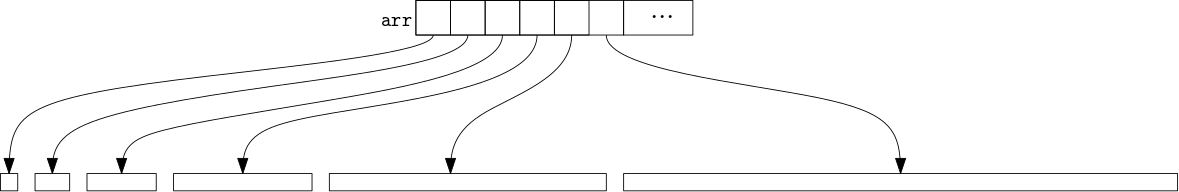
\includegraphics[width=6.5in]{pics/doublingArray.png}
  \caption{Array Segments}
  \label{fig::doublingArray}
\end{figure}

\paragraph{Garbage Collection}
We did not handle garbage collection: \nf{Enqueue} operations  remain in the nodes even after their elements have been dequeued.
We can keep track of the \nf{block}s in the \nf{root} whose operations are all terminated, i.e, all of its enqueues have been dequeued and the responses of all of its dequeues have been computed. We call these blocks \it{finished blocks}. If we help the operations of all processes to compute their responses, then we can say if block $B$ is finished then all blocks before $B$ are also finished. Knowing the most recent finished block in a node we can reclaim the memory taken by finished blocks. To throw the garbage in the blocks away we cannot use arrays (or vectors). We need a data structure that supports \nf{tryAppend()}, \nf{read(i)}, \nf{write(i)} and \nf{split(i)} operations in $O(\log n)$. Where \nf{split(i)} removes all the indices less than \nf{i}. We can use a concurrent implementation of persistent red black trees for this~\cite{DBLP:conf/podc/BashariW21}.

\begin{figure}[hbt]  
  \center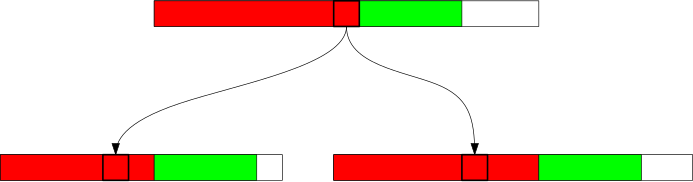
\includegraphics[width=3.5in]{pics/finishedBlocks.png}
  \caption{Finished blocks are shown with red color and unfinished blocks are shown with green color. All the subblocks of a finished block are also finished.}
  \label{fig::doublingArray}
\end{figure}

\paragraph{Poly-logarithmic Wait-free Sequences}
Consider a data structure storing a sequence that supports three operations \nf{append(e)}, \nf{get(i)} and \nf{index(e)}. An \nf{append(e)} adds \nf{e} to the end of the sequence, a \nf{get(i)} gets the \nf{i}th element in the sequence and an \nf{index(e)} computes the position of element \nf{e} in the sequence. We can modify our queue to design such data structure. \nf{append(e)} is implemented like \nf{Enqueue(e)}, \nf{get(i)} is done by calling \nf{DSearch} with replacing the \nf{BinarySearch} on the entire \nf{root.blocks} array and \nf{index(e)} is done similarly to \nf{IndexDequeue} (except operating on enqueues instead of dequeues).
 We achieve this with poly-logarithmic steps for each operation with respect to the number of \nf{append}s done.

\paragraph{Stacks}
There are two reasons block tree worked well to implement a queue. Firstly, to respond to a \nf{Dequeue} we do not need to look at the entire history of operations: if a \nf{Dequeue} does not return\nf{null} we can compute the index of the \nf{Enqueue} that is its response in $O(\log n)$ time if we keep the number of enqueues and the size. Secondly, the operations we need to search to respond to the \nf{Dequeue} is not very far from it in the sequence of operations: the distance is at most linear in the size of the queue. It may be possible to create wait-free poly-logarithmic implementaion of other objects whose operations satisfy these two conditions. 

\pagebreak

\bibliography{main.bib} 
\bibliographystyle{plain}

\end{document}

